\section{Limits, colimits, and adjunctions}\label{906}
Hi! This is 18.906. I'm glad to see familiar faces, and new faces. Let me introduce the course. It's a pset based course, with 6 psets. The first one is due Feb 22. It's due every two weeks, so I can't formulate all porblems right at the beginning of the two weeks. I'll try to have the psets done a week before the psets are due. So the first couple problems are up for this pset. You'll be glad to hear that there's no final. I don't think I'll do it again, not this term.

I'll have office hours every week, but I don't know when yet. Hood's the grader and he'll have office hours. There's a course website which can be easily found. What's the course about? Really homotopy theory. 905 was homology and cohomology. Here's the table of contents.
\begin{enumerate}
    \item General homotopy theory (category theory). Because it started in algtop, I have the right to talk about it here. Homotopy groups, lexseqs, obstruction theory.
    \item Bundles. The theme of the course is using bundles to understand spaces. Brown representability, classifying spaces.
    \item Spectral sequences(!!!) The story is that it was invented as a piece of algtop. But in the last 60 years it's become a general mathematical tool.
    \item Homotopy-theoretic applications. How to relate homotopy and homology (Hurewicz, whitehead, and local versions like mod C).
    \item Characteristic classes (Thom, Euler, Chern, Steifel-Whitney class), where applications to geometry come in.
    \item Time permitting, there's a beautiful story that comes out (on cobordism, etc).
\end{enumerate}
Any questions? I try to correspond problems in the psets and lectures.
\subsection{Category theory}
I'm interested in ``construction''. In 905, I began by talking about category theory. I just won't introduce basic concepts again. Suppose $\cI$ is a small category (a set of objects), and $\cc$ another category.
\begin{definition}
    Let $X:\cI\to\cc$. A cone under $X$ is a natural transformation from $X$ to a constant functor. So for every $f:i\to j$ in $\cI$, the diagram should commute:
    \begin{equation*}
	\xymatrix{
	    X_i\ar[d]^{f_\ast}\ar[dr]^{f_i} & \\
	    X_j\ar[r]^{f_j} & Y
	    }
    \end{equation*}
    A \emph{colimit} of $X$ is an initial cone under $X$. So, for all $(Y,f_i)$, there exists a unique $h:L\to Y$ such that $h\circ g_i = f_i$.
\end{definition}
For example, we can let $\cI = \mathbf{N}$ made a category via its natural poset structure. For example, if $\cc = \mathbf{Ab}$, then you can consider $\Z\xrightarrow{2}\Z\xrightarrow{3}\Z\to\cdots$. The colimit of this is $\QQ$, where the maps are:
\begin{equation*}
    \xymatrix{
	\Z\ar[r]^2\ar[dr]^1 & \Z\ar[r]^3\ar[d]^{1/2} & \Z\ar[r]^4\ar[dl]^{1/3!} & \cdots\\
	& \QQ & &
    }
\end{equation*}
It looks pretty initial, doesn't it?

For example, if $\cI = G$ and $\cc=\Top$, then this is just a group action on a topological space. The colimit of this functor is the orbit space, i.e., $X/G$ (technically this is $G\backslash X$ because $G$ acts on the left).

How about the following $\cI$:
\begin{equation*}
    \xymatrix{
	& b\\
	a\ar[ur]\ar[dr] & \\
	& c
    }
\end{equation*}
and $\cc=\Top$. The cone of this is the pushout $B\cup_A C:= B\sqcup C/\sim$ where $f(a)\sim g(a)$ for all $a\in A$! Basically, you're gluing $B$ and $C$ along $A$. For example, attaching cells to CW-complexes. If the category is groups, then the pushout is Instead of the disjoint union, you take the free product, and then quotient out to get something known as the \emph{amalgamated free product}.

If you had the following $\cI$:
\begin{equation*}
    \begin{tikzcd}
	a\ar[r,shift left=.75ex]\ar[r,shift right=.75ex] & b
    \end{tikzcd}
\end{equation*}
The colimit of this in any category is what's called the \emph{coequalizer}.

Similarly, if $\cI$ is a discrete category (only a set, with identity maps). The colimit is the coproduct. If the category is sets, or spaces, this is the disjoint union. If the category is abelian groups, then one option would be the product. But this only works if $\cI$ is finite. A better thing is to take the (possibly infinite) direct sum.

\begin{remark}
    Analogously, you can consider \emph{cones over} $X$. While Miller defined this in class, I'll leave it you, beloved reader, to figure out this definition. It's really just a cone in the opposite category. Like the notion of a colimit, we get a limit as a terminal object in cones over $X$. I encourage you to consider limits in the examples above. For example, in the second example above, the limit of a group action is the fixed point set!
\end{remark}
So products are limits, for example. Think about this yourself, because I want to talk about one more thing, namely adjoint functors.
\subsection{Adjoint functors}
This is a very useful concept. We have an example, already. Let $\cc^\cI = \Fun(\cI,\cc)$. We've been working in this category! Ok, so what we have is a functor $\cc\to \cc^\cI$, given by the constant functor. We also have a functor $\cc^\cI\to \cc$ given by the colimit. This may not exist in general, but in our examples above, they always exist. What's the rule this colimit plays? Well:
$$\cc(\colim_{i\in \cI} X_i,Y) = \cc^\cI(X,\mathrm{const}_Y)$$
where $X:\cI\to\cc$. This is reminiscent of the adjunction operator in linear algebra. So this is an example of an adjoint functor. In fact, also:
$$\cc(W,\lim_{i\in \cI} X_i) = \cc^{\cI}(\mathrm{const}_W,X)$$
Another adjunction where the constant functor functor (yes, two ``functor''s!) appears on the left!
\begin{definition}[Invented by Dan Kan, late, of this department]
    Let $\cc,\cd$ be categories. Let $F:\cc\to \cd$ and $G:\cd\to\cc$. An \emph{adjunction} between $F$ and $G$ is an isomorphism:
    $$\cd(FX,Y) = \cc(X,GY)$$
    which is natural in $X$ and $Y$. We say that $F$ is a left adjoint of $G$ and $G$ is a right adjoint of $X$. People typically write left adjoints on the top.
\end{definition}
For example, there's a forgetful functor $\mathrm{Grp}\to\mathrm{Set}$. Any set determines a group. Hmm. What is this? Set maps $X\to u\Gamma$ should be the same as group maps $FX\to \Gamma$ where $\Gamma$ is a group and $F$ is our mysterious left adjoint. $u$ is the forgetful functor. So $FX$ is the free group! This is literally the definition of the free group.
\begin{definition}
    $\cc$ is \emph{cocomplete} if all colimits exist. It's \emph{complete} if all limits exist.
\end{definition}
Obviously I'm talking about small (co)limits. If a functor has both left and right adjoints, it's super nice! We'll reconvene on Friday.

\section{Compactly generated spaces}
A lot of the course is going to be about loop spaces, and mapping spaces. Standard topology doesn't do very well with mapping spaces. So we are going to narrate the story of compactly generated spaces. One of the good things is that you have a \emph{Cartesian-closed category}.

The first thing I want to talk about is the Yoneda lemma. We will start to do some topology pretty soon. OK, so I was proposing the notion of a colimit of a functor. It was defined in terms of maps out of the colimit. More precisely:
$$\cc(\colim_{j\in\cJ}X_j,Y) = \cc^\cJ(X_\bullet,\mathrm{const}_Y)$$
They're naturally isomorphic, and that's all you can ask for in this life. How well-defined is this object, if it exists? Whether it exists is a question of how cocomplete your category is. The question of uniqueness is more general. Let's think about that for a minute. The Yoneda lemma -- sometimes ``you-need-a-lemma''(!!) -- is:
\begin{theorem}[Yoneda lemma]
    Consider the functor $\cc(X,-):\cc\to\set$. Suppose $G:\cc\to\set$ is another functor. It turns out that:
    $$\mathrm{nt}(\cc(X,-),G)\simeq G(X)$$
\end{theorem}
\begin{proof}
    Let $x\in G(X)$. We then define a natural transformation that sends $f:X\to Y$ to $f_\ast(x)\in G(Y)$. On the other hand, suppose $\theta:C(X,-)\to G$. Send $\theta$ to $\theta_X(1_X)$. These two are so natural and beautiful that you expect that they're inverses, right? And they are.
\end{proof}
OK, so in particular if $G=\cc(Y,-)$ -- these are called \emph{corepresentable} functors -- then $\mathrm{nt}(\cc(X,-),\cc(Y,-))\simeq \cc(Y,X)$. What this means is that if you look at natural isomorphisms $\cc(X,-)\to \cc(Y,-)$, that's the same as isomorphisms $Y\to X$. This means that if you have a corepresentable functor, the object that represents is unique\footnote{at least up to isomorphism}.
\subsection{CGHW spaces}
Some constructions commute for ``categorical reasons''. Here's the example to keep in mind. Let $X\in \Top$. Then $X\times\lim_{j\in\cJ}Y_j\simeq \lim_{j\in\cJ}(X\times Y_j)$. Why? This is easily proven because both the limit and the product are defined by what maps into them are. In contrast, $X\times\colim_{j\in \cJ}Y_j$ is not $\colim_{j\in \cJ}(X\times Y_j)$ in general. Very sad :-( An example of this failure is a quotient map $Y\to Z$. Then $X\times Y\to X\times Z$, is this a quotient map? It's not true in general. It's a very sad state of affairs.
\begin{theorem}[Whitehead]
    It is if $X$ is a compact Hausdorff space.
\end{theorem}
I want to repair that problem. Why were we talking about colimits? Here's an observation. Suppose $X\to Y$ is a quotient map; then a map $Y\to Z$ is continuous iff the composite $X\to Y\to Z$ is continuous. A quotient map \emph{is} a coequalizer. What I'm saying is, I can find two maps to $X$ such that $Y$ is a coequalizer of $X$. What space are we mapping into $X$? Well, suppose $Z=X/\sim$. If we considered:
\begin{equation*}
    \begin{tikzcd}
	X\times_Z X\ar[r,shift left=.75ex,"\pi_1"]\ar[r,shift right=.75ex,swap,"\pi_2"] & X\ar[r] & Z
    \end{tikzcd}
\end{equation*}
The term here is ``regular epimorphism''.

\begin{remark}
    OK, the statement about limits and products is wrong. Think about what happens when $\cJ$ is a discrete category. We will fix this on Monday.
\end{remark}

We don't want to just restrict ourselves to compact Hausdorff spaces. So we look at topologies detected by maps from compact Hausdorff spaces.
\begin{definition}
    Let $X$ be a space. A subspace $F\subseteq X$ is called \emph{compactly closed} if for any map $k:K\to X$ from compact Hausdroff $K$, then $k^{-1}(F)\subseteq K$ is closed.
\end{definition}
If $F$ is closed, then it's clearly compactly closed. But there might be non-closed compactly closed sets.
\begin{definition}
    $X$ is a $k$-space if compactly closed implies closed.
\end{definition}
The $k$ comes from ``kompact'' and/or Kelly, an early topologist who considered this stuff.

Let $X$ be any space. It can be $k$-ified to some space denoted $kX$. You just enlarge the topology so that it includes the compactly closed sets. This is a topology, bigger than the original one. So the identity $kX\to X$ is continuous.

\begin{remark}
    $X$ is a $k$-space iff it has the property that a map $X\to Y$ is continuous iff for any compact Hausdorff $K$ and map $k:K\to X$, the composite $K\to X\to Y$ is continuous.
\end{remark}
\begin{example}
    Compact Hausdorff spaces are $k$-spaces. First countable (so metric spaces) and CW-complexes are also $k$-spaces.
\end{example}
Define $k\Top$ to be the category of $k$-spaces. There's an inclusion $i:k\Top\hookrightarrow \Top$. Now $k$-ification gives a functor $\Top\to k\Top$. This has the property that:
$$k\Top(X,kY)=\Top(iX,Y)$$
Here's an adjunction! This means that $k(iX\times iY)=X\times^{k\Top}Y$ where $X$ and $Y$ are $k$-spaces. It's true that $kiX\simeq X$.

The takeaway is that $k\Top$ has good categorical properties inherited from $\Top$, i.e. it's complete and cocomplete. I want to now talk about mapping spaces, which shows that $k\Top$ is even better!
\subsection{Mapping spaces}
Let $X$ and $Y$ be spaces. There's the compact-open topology on $\Top(X,Y)$. For $k$-spaces, I want to make a slight modification. In particular, if $X$ and $Y$ are $k$-spaces, define a topology on $k\Top(X,Y)$ generated by: $W(k:K\to X, \text{ open }U\subseteq Y)=\{f:X\to Y: f(k(K))\subseteq U\}$. We write $Y^X$ for the $k$-ification of this space.
\begin{prop}
    \begin{enumerate}
	\item $(k\Top)^{op}\times k\Top\to k\Top$ given by $(X,Y)\to Y^X$ is a functor of both variables.
	\item $e:X\times Z^X\to Z$ given by $(x,f)\mapsto f(x)$ and $i:Y\to (X\times Y)^X$ given by $y\mapsto(x\mapsto(x,y))$ are continuous.
    \end{enumerate}
\end{prop}
\begin{proof}
    Look online -- there are references on the webpage.
\end{proof}
I'm not where I wanted to be at this moment in time. Ok, here's a result of this proposition. Consider $k\Top(X\times Y,Z)$ where the product is the product in $k$-spaces. What is $k\Top(Y,Z^X)$? I want to say that:
$$k\Top(X\times Y,Z)\simeq k\Top(Y,Z^X)$$
defined by $(f:X\times Y\to Z)\mapsto (Y\xrightarrow{i}(X\times Y)^X\to Z^X)$ in one direction, and by $(f:Y\to Z^X)\mapsto(X\times Y\to X\times Z^X\xrightarrow{e} X)$. They're so natural that they have to be inverses to one another. Let me close with a definition.
\begin{definition}
    A category $\cc$ with finite products is Cartesian closed if for any $X$, the functor $X\times -:\cc\to \cc$ has a right adjoint.
\end{definition}
So $k\Top$ is Cartesian closed, but $\Top$ isn't. On Monday, I'll justify why this is important.
\section{``Cartesian closed'', Hausdorff, Basepoints}
Pset 1 is up, and there's now a number 4. My office hours are Tuesday from 12 to 1:30 in 2-478.

Remember that I wrote something that's obviously wrong; let $Y:\cI\to\cc$. I claimed that $\lim_\cI (X\times Y_i)\simeq X\times \lim_\cI Y_i$. This isn't right because if $\cI$ is a discrete category, this doesn't make sense. One way to fix this is implemented in problem 4. Another way is, let $X:\cI\to\cc$. Then I can take $\lim_\cI(X_i\times Y_i)$, and this is $\lim_\cI X_i\times \lim_\cI Y_i$. This is part of a more general picture involving a Frobenii theorem. You can find out more from MacLane's book or something.

I want to catch up with something that I had to say before but I didn't. That's the relationship between (co)limits and adjoint functors. Namely, left adjoints respect colimits and right adjoints respect limits. There's something called the adjoint functor theorem. For example, $Y\times -:\Top\to\Top$. One kind of colimit is the pushout $X/A=X\cup_A \ast$. But $Y\times X\cup_{Y\times A}\ast\simeq (Y\times X)/(Y\times A)$. But this isn't the same as $Y\times (X/A)$! There is a bijective map $Y\times X/Y\times A\to Y\times(X/A)$, but it's not a homeomorphism in general. The reason this fails is because $Y\times -$ is \emph{not} a left adjoint!

But it is a left adjoint when working with compactly generated spaces (i.e., $k$-spaces)\footnote{Compactly generated spaces are weakly Hausdorff $k$-spaces, what Professor Miller said here was incorrect.}! Recall that this means that $k\Top$ is Cartesian closed. We're gonna make a lot of use of the space $Z^X:=k(k\Top(X,Z))$. You'll check that $(X,Z)\mapsto Z^X$ is a functor. Another thing is that $Z^{X\times Y}\simeq (Z^X)^Y$ and $(Y\times Z)^X\simeq Y^X\times Z^X$. There's a composition map $Y^X\times Z^Y\to Z^X$.

When the ancients came up with the definition of a topology, they were good axioms -- but these are better! Sometimes, you want even more, e.g., points being closed. There's a further refinement of $k$-spaces. 
\subsection{``Hausdorff''}
\begin{definition}
    A space is ``weakly Hausdorff'' if the image of every map $K\to X$ from a compact Hausdorff space $K$ is closed.
\end{definition}
Another way to say this is that the map itself if closed. Clearly Hausdorff implies weakly Hausdorff. Another thing this means is that every point in $X$ is closed (eg $K=\ast$). 
\begin{prop}
    Let $X$ be a $k$-space.
    \begin{enumerate}
	\item $X$ is weakly Hausdorff iff $\Delta:X\to X\times^k X$ is closed. In algebraic geometry such a condition is called separated.
	\item Let $R\subseteq X\times X$ be an equivalence relation. If $R$ is closed, then $X/R$ is weakly Hausdorff.
    \end{enumerate}
\end{prop}
\begin{definition}
    A space is comapctly generated if it's a weakly hausdorff $k$-space. The category of such spaces is called $\CG$.
\end{definition}
We have a pair of adjoint functors $(i,k):\Top\to k\Top$. It's possible to define a functor $k\Top\to \CG$ given by $X\mapsto X/\bigcap\text{all closed equivalence relations}$. It is easy to check that if $Z$ is weakly Hausdorff, then $Z^X$ is weakly Hausdorff (where $X$ is a $k$-space). What this implies is that $\CG$ is also Cartesian closed!

I'm getting a little tired of point set stuff. Let's start talking about homotopy and all that stuff today for a bit. You know what a homotopy is. I will not worry about point-set topology anymore. So when I say $\Top$, I probably mean $\CG$. A homotopy between $f,g:X\to Y$ is a map $h:I\times X\to Y$ such that the following diagram commutes:
\begin{equation*}
    \xymatrix{
	X\ar[dr]_{i_0}\ar[drr]^f & &\\
	& I\times X\ar[r]^h & Y\\
	X\ar[ur]^{i_1}\ar[urr]_g & &
    }
\end{equation*}
We write $f\sim g$. We define $[X,Y]=\Top(X,Y)/\sim$. Well, a map $I\times X\to Y$ is the same as a map $X\to Y^I$ but also $I\to Y^X$. The latter is my favorite! It's a path of maps from $f$ to $g$. So $[X,Y]=\pi_0Y^X$.

To talk about higher homotopy groups and induct etc. we need to talk about basepoints.
\subsection{Basepoints}
A pointed space is $(X,\ast)$ with $\ast\in X$. This gives a category $\Top_\ast$ where the morphisms respect the basepoint. This has products because $(X,\ast)\times (Y,\ast)=(X\times Y,(\ast,\ast))$. How about coproducts? It has coproducts as well. This is the wedge product, defined as $X\sqcup Y/\ast_X\sim \ast_Y=:X\vee Y$. This is \verb|\vee|, not \verb|\wedge|. Is this category also Cartesian closed?

Define the space of pointed maps $Z^X_\ast\subseteq Z^X$ topologized as a subspace. Does the functor $Z\mapsto Z^X_\ast$ have a left adjoint? Well $\Top(W,Z^X)=\Top(X\times W,Z)$. What about $\Top(W,Z^X_\ast)$? This is $\{f:X\times W\to Z:f(\ast,w)=\ast\forall w\in W\}$. That's not quite what I wanted either! Thus $\Top_\ast(W,Z^X_\ast)=\{f:X\times W\to Z:f(\ast,w)=\ast=f(x,\ast)\forall x\in X, w\in W\}$. These send both ``axes'' to the basepoint. Thus, $\Top_\ast(W,Z^X_\ast)=\Top_\ast(X\wedge W,Z)$ where $X\wedge W=X\times W/X\vee W$ because $X\vee W$ are the ``axes''.

So $\Top_\ast$ is not Cartesian closed, but admits something called the smash product\footnote{Remark by Sanath: this is like the tensor product.}. What properties would you like? Here's a good property: $(X\wedge Y)\wedge Z$ and $X\wedge(Y\wedge Z)$ are bijective in pointed spaces. If you work in $k\Top$ or $\CG$, then they are homeomorphic! It also has a unit.

Oh yeah, some more things about basepoints! So there's a canonical forgetful functor $i:\Top_\ast\to \Top$. Let's see. If I have $\Top(X,iY)=\Top_\ast(??,Y)$? This is $X_+=X\sqcup \ast$. Thus we have a left adjoint $(-)_+$. It is clear that $(X\sqcup Y)_\ast = X_+ \vee Y_+$. The unit for the smash product is $\ast_+ = S^0$.

On Friday I'll talk about fibrations and fiber bundles.
\section{Fiber bundles, fibrations, cofibrations}
My office hours are Tuesday, 12 - 1:30 and Hood's are Tuesday, 12(next week). It'll probably be Mondays in the future, at 12 as well. Next Monday is a holiday, and next Tuesday is a Monday. Oh, pset 1 is due on Wednesday.

Today's gonna be about fiber bundles and fibrations and possibly cofibrations as well. This is proper homotopy theory.  You have probably seen fiber bundles before. Do you like the yellow chalk? I think it looks good.
\begin{definition}[Fiber bundles]
    A fiber (or fibre, if you're British) bundle is a map (of compactly generated spaces, \emph{always} -- although every space in nature is already a weakly Hausdorff $k$-space; it's not a big deal!) $p:E\to B$ such that for every $b\in B$, there exists an open $U\subseteq B$ such that $b\in U$, and a map $p^{-1}(U)\to p^{-1}(b)$ such that $p^{-1}(U)\to U\times p^{-1}(b)$ is a homeomorphism.
\end{definition}
So the preimage over every point looks like a product. So it's locally trivial in the base. Of course, there's an alternate way to say this. Equivalently, there is an open cover $\cU$ (called the \emph{trivializing cover}) of $B$ such that for every $U\subseteq \cU$, there is a space $F$ and a homeomorphism $p^{-1}(U)\simeq U\times F$ that's compatible with the projections down to $U$.
\begin{remark}
    We say that $E$ is the total space, $B$ is a base space, $p$ is a projection, and $F$ (which can vary) -- actually I'll write $p^{-1}(b)$ -- is called the fiber over $b$.
\end{remark}
\begin{example}
    You know of many examples. A covering space $E\to B$ is a fiber bundle with discrete fibers. Thus fiber bundles generalize covering spaces to more interesting cases.
\end{example}
\begin{example}
    The Hopf fibration. It's a fiber bundle. We have $S^3\subseteq \cc^2$. And, well, we can consider the map $S^3\to \CP^1$ that sends a vector through the complex line through $v$. Now, $\CP^1\simeq S^2$. So you have a non-nullhomotopic map $S^3\to S^2$. Here's a picture of this. (I cannot livetex this)

    The Hopf fibration is a map between smooth manifolds. This is a great way to construct fibrations.
\end{example}
\begin{theorem}[Ehresmann]
    Suppose $E$ and $B$ are smooth manifolds, and let $p:E\to B$ be a smooth (i.e., $C^\infty$) map. Then $p$ is a fiber bundle if:
    \begin{enumerate}
	\item It's a submersion (so $dp:T_e E\to T_{p(e)} B$ is a surjection)
	\item $p$ is proper, so preimages of compact sets are compact.
    \end{enumerate}
\end{theorem}
For example, I can look at the complement of a closed set in $S^3$, and then the restriction of $p$ won't be a fiber again.

The whole course is about fiber bundles, namely about its cohomological and homotopical structure.

\begin{definition}[See Peter May's \emph{Concise Course}]
   Let $X$ be a space. Say that an open cover $\cU$ is \emph{numerable} if there exists a subordinate partition of unity, i.e., for each $U\in\cU$ we're given $f_U:X\to [0,1]=I$ such that $f^{-1}((0,1]) = U$ and any $x\in X$ belonds to only finitely many $U\in\cU$.

    Say that $X$ is paracompact if any open cover admits a numerable refinement.
\end{definition}
\begin{example}
    CW-complexes are paracompact.
\end{example}
The numerable definition is technical, but you're really just restricting the class of coverings you're looking at.
\begin{definition}
    A fiber bundle is ``numerable'' if it admits a numerable trivializing cover.
\end{definition}

Fiber bundles are still too narrow. So I will now tell you what a fibration is.

\begin{definition}
    A map $p:E\to B$ is called a \emph{Hurewicz fibration} (I'll just say fibration) if it satisfies the homotopy lifting property (HLP). That says this. Suppose I have a homotopy $h:I\times W\to B$. Then there exists a lift:
    \begin{equation*}
	\xymatrix{
	    W\ar[r]^f\ar[d]_{\mathrm{in}_0} & E\ar[d]^p\\
	    I\times W\ar[r]_h\ar@{-->}[ur]^{\overline{h}} & B
	    }
    \end{equation*}
    Where the outer diagram commutes. It doesn't need to be a unique lift!
\end{definition}
This is an extremely alarming definition. This has to be checked for all spaces and all maps and all homotopies! So it took an act of genius to construct something like this. The idea of doing something like this goes back to Serre back in about 1950. It solved a problem (of defining what a fibration was).

But it's not impossible to check! Let me tell you some stuff. Hurewicz was a faculty member here, one of the first algebraic topologists here. I'm going to try to reformulate this diagram here a little bit. Let me try to adjoint the $I$. Then I have:
\begin{equation*}
    \xymatrix{
	E\ar[r]^p & B\\
	W\ar[u]^f\ar[r]_{\widehat{h}} & B^I\ar[u]_{\mathrm{ev}_0}
    }
\end{equation*}
This is just the adjoint of our diagram. Now, a diagram like this is the same as a map $W\to B^I\times_B E$ (the pullback is the set of paths and points $(\omega, e)$ such that $\omega(0) = p(e)$. But now, if our dotted map exists, we'd have a lifted homotopy $\widehat{\overline{h}}:W\to E^I$. We have a map $\widetilde{p}:E^I\to B^I\times_B E$ given by $\omega\mapsto (p\omega,\omega(0))$. Clearly $p\omega(0) = p\omega(0)$, so this lands in $B^I\times_B E$.

Thus the existence of $\overline{h}$ is the same as a lift:
\begin{equation*}
    \xymatrix{
	& E^I\ar[d]^{\widetilde{p}}\\
	W\ar[r]\ar@{-->}[ur]^{\widehat{\overline{h}}} & B^I\times_B E
    }
\end{equation*}
Obviously the universal example is $B^I\times_B E$. If $p$ is a fibration, then I can make the lift in the following diagram, and if I can lift for any $W$, I can obviously construct the lift in the following diagram:
\begin{equation*}
    \xymatrix{
	& E^I\ar[d]^{\widetilde{p}}\\
	B^I\times_B E\ar@{-->}[ur]^\lambda\ar[r]^1 & B^I\times_B E
    }
\end{equation*}
We say $\lambda$ is a \emph{lifting function}. Well, if $\omega(0) = p(e)$, then $\lambda(\omega:I\to B, e\in E):I\to E$. And in particular, $p\circ\lambda(\omega, e) = \omega$ and $\lambda(\omega,e)(0) = e$. So $\lambda$ starts with a path $\omega$ in $B$, and some point over the starting point, and produces a path in $E$ which lives over $\omega$. In other words, it's a path lifting. The key thing is that it's a continuous way to lift. So you \emph{can} check the HLP in certain cases.
\begin{theorem}[Dold]
    Let $p:E\to B$ be a map. Assume there's a numerable cover of $B$, say $\cU$, such that for every $U\in\cU$, the restriction $p|_{p^{-1}(U)}:p^{-1}U\to U$ is a fibration. (It's locally a fibration over the base). Then $p$ itself is a fibration.
\end{theorem}
Check for yourself that at least a product projection $\mathrm{pr}_1:B\times F\to B$ is a product fibration (e.g. using the universal property or something). So in particular, \emph{every numerable fiber bundle is a fibration}. I.e., numerable fiber bundles satisfy the homotopy lifting property. We'll see why this is such a good thing next week. Questions?
\section{Fibrations and cofibrations}
Recall that fibrations are maps $p:E\to B$ such that for every $W$ there is a lift:
\begin{equation*}
    \xymatrix{
	W\ar[r]\ar[d]_{in_0} & E\ar[d]^p\\
	W\times I\ar[r]\ar@{-->}[ur] & B
    }
\end{equation*}
Here is a rather simple result to show.
\begin{prop}
    \begin{enumerate}
	\item Fibrations are closed under pullbacks. In other words, if $p:E\to B$ is a fibration and $X\to B$ is any map, then the induced map $E\times_B X\to X$ is a fibration.
	\item Fibrations are closed under exponentiation and products. In other words, if $p:E\to B$ is a fibration, then $E^A\to B^A$ is another fibration.
	\item Fibrations are closed under composition.
    \end{enumerate}
\end{prop}
\subsection{Comparing fibers over different points in $B$}
OK, let's consider a path $\omega:I\to B$ with $\omega(0) = a$ and $\omega(1) = b$. Let $F_a$ be the fiber over $a$. Then we want to have a map $F_a\to F_b$, because of our considerations on liftings of paths. How do we get such a map?

Consider the diagram:
\begin{equation*}
    \xymatrix{
	F_a\ar[d]_{in_0}\ar[rr] & & E\ar[d]^p\\
	I\times F_a\ar@{-->}[ur]^{h}\ar[r]_{pr_1} & B\ar[r]_{\omega} & B
    }
\end{equation*}
Does this diagram commute? Yes, because $\omega(0) = a$. Thus, by the homotopy lifting property, the dotted arrow exists. Now, if $x\in F_a$, then $h(1,x) \in F_b$ and $h(0,x) = x$. Thus we get a map $f:F_a\to F_b$ where $f(x) = h(1,x)$.

Great! Now the question we can ask is: how unique if $f$? Namely, if we have two homotopic paths $\omega_0,\omega_1$ with $\omega_0(0) = \omega_1(0) = a$ and $\omega_0(1) = \omega_1(1) = b$, with a given homotopy $g:I\times I\to B$, how do $f_0$ and $f_1$ relate?

We have a diagram of the form:
\begin{equation*}
    \xymatrix{
	((\partial I\times I)\cup (I\times 0))\times F_a\ar[d]_{in_0}\ar[rr] & & E\ar[d]^p\\
	I\times I\times F_a\ar[r]_{pr_1}\ar@{-->}[urr] & I\times I\ar[r]_g & B
    }
\end{equation*}
Think of the space $(\partial I\times I)\cup (I\times 0)$ as follows:
\begin{equation*}
\begin{tikzpicture}
    \draw (2,2) -- (0,2) -- (0,0) -- (2,0);
    \node [above] at (1,2) {$h_1$};
    \node [below] at (1,0) {$h_0$};
    \node [left] at (0,1) {$in_0$};
\end{tikzpicture}
\end{equation*}
and $I\times I$ looks like:
\begin{equation*}
    \begin{tikzpicture}
	\draw (0,0) -- (0,2) -- (2,2) -- (2,0) -- (0,0);
	\draw[fill] (2,2) circle [radius=0.05];
	\draw[fill] (2,0) circle [radius=0.05];
	\node [left] at (0,1) {$a$};
	\node [above] at (1,2) {$\omega_1$};
	\node [below] at (1,0) {$\omega_0$};
	\node [right] at (2,1) {$b$};
	\node [above right] at (2,2) {$f_1$};
	\node [below right] at (2,0) {$f_0$};
    \end{tikzpicture}
\end{equation*}

Does the dotted map exist? Clearly this is crying out for us to use the homotopy lifting property. But what should our space $W$ be? Well the following pair:
\begin{equation*}
    \begin{tikzpicture}
	\draw (2,2) -- (0,2) -- (0,0) -- (2,0);
    \end{tikzpicture}\subseteq
    \begin{tikzpicture}
	\draw (0,0) -- (0,2) -- (2,2) -- (2,0) -- (0,0);
    \end{tikzpicture}
\end{equation*}
is homotopy equivalent to $(0\subseteq I)\times I$. Hence in our diagram we now have:
\begin{equation*}
    \xymatrix{
	I\times F_a\ar[r]|{\simeq} & ((\partial I\times I)\cup (I\times 0))\times F_a\ar[d]_{in_0}\ar[rr] & & E\ar[d]^p\\
	I\times I\times F_a\ar[r]_{\simeq} & I\times I\times F_a\ar[r]_{pr_1}\ar@{-->}[urr] & I\times I\ar[r]_g & B
    }
\end{equation*}
This whole diagram commutes; letting $W=I\times F_a$ thus gives us the desired lift. Restricting to the right side of the C-shaped region (which the HLP says can be completed to a square) gives a homotopy $f_0\simeq f_1$. Thus liftings of homotopic paths are unique up to homotopy. How do we express this functorially?
\subsection{Fundamental groupoid}
\begin{definition}
    Given a space $X$, the fundamental groupoid is a category (in fact, groupoid) denoted $\Pi_1(X)$, whose objects are points of $X$ and maps are homotopy classes of paths in $X$. Composition of compatible $\sigma$ and $\omega$ is the path:
    \begin{equation*}
	(\sigma\cdot\omega)(t) = \begin{cases}
	    \omega(2t) & 0\leq t\leq 1/2\\
	    \sigma(2t - 1) & 1/2\leq t\leq 1
	\end{cases}
    \end{equation*}
\end{definition}
What we've therefore showed is:
\begin{prop}
    Any fibration $p:E\to B$ gives a functor $\Pi_1(B)\to \Top$.
\end{prop}
This is the beginning of a beautiful story involving fibrations. If you're interested, look up ``Grothendieck construction''.
\subsection{Cofibrations}
Let's turn to a different question. Let $i:A\to X$. When is $Y^X\to Y^A$ a fibration? Well, we want a lifting:
\begin{equation*}
    \xymatrix{
	W\ar[r]\ar[d]_{in_0} & Y^X\ar[d]\\
	I\times W\ar@{-->}[ur]\ar[r] & Y^A
    }
\end{equation*}
This can be adjointed over to get:
\begin{equation*}
    \xymatrix{
	A\times W\ar[r]^{i\times 1}\ar[d]_{1\times in_0} & X\times W\ar[d]\ar[ddr]& \\
	A\times W\times I \ar[r]\ar[drr] & X\times I\times W\ar@{-->}[dr] & \\
	& & Y
    }
\end{equation*}
Adjointing over again:
\begin{equation*}
    \xymatrix{
	A\ar[r]\ar[d] & X\ar[d]\ar[ddr] & \\
	A\times I\ar[r]\ar[drr] & X\times I\ar@{-->}[dr] & \\
	& & Y^W
    }
\end{equation*}
This motivates the following definition of something that's \emph{dual} to the notion of fibration:
\begin{definition}
    $i:A\to X$ is a \emph{cofibration} if it satisfies the \emph{homotopy extension property}, i.e. for all solid arrow diagrams, the following diagram commutes for any $Y$:
    \begin{equation*}
    \xymatrix{
	A\ar[r]\ar[d] & X\ar[d]\ar[ddr] & \\
	A\times I\ar[r]\ar[drr] & X\times I\ar@{-->}[dr] & \\
	& & Y
    }
    \end{equation*}
\end{definition}
The universal example is the pushout $X\cup_A (A\times I)$. So, equivalently, we're asking for the existence of a dotted arrow:

\begin{equation*}
    \xymatrix{
	X\cup_A (A\times I)\ar[r]\ar[dr] & X\times I\ar@{-->}[d]\\
	& Z
    }
\end{equation*}
for any $Z$. But this is equivalent to the existence of a dotted arrow in the following diagram:
\begin{equation*}
    \xymatrix{
	X\cup_A (A\times I)\ar[r]\ar[dr] & X\times I\ar@{-->}[d]\\
	& X\cup_A(A\times I)\ar[d]\\
	& Z
    }
\end{equation*}
This is in turn equivalent to asking that $X\cup_A (A\times I)$ is a retract of $X\times I$.

\begin{example}
    $S^{n-1}\hookrightarrow D^n$ is a cofibration.
    \begin{figure}[H]
	\centering
	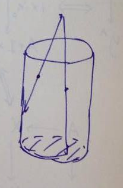
\includegraphics[scale=0.75]{retract-cofibration}
	\caption{Drawing by John Ni.}
    \end{figure}
\end{example}
In particular, $\{0,1\}\hookrightarrow I$ is a cofibration.
\section{Homotopy fibers, the Barratt-Puppe sequence}
Yesterday, I showed this:
\begin{prop}
    If $A\to X$ is a cofibration, then for any $Y$, the map $Y^X\to Y^A$ is a fibration.
\end{prop}
We did this by reverse-engineering.
\begin{example}
    $S^{n-1}\hookrightarrow D^n$ is a cofibration.
\end{example}
Let me point out properties of cofibrations.
\begin{itemize}
    \item It's closed under cobase change. What this means is if I have a cofibration $A\to X$ and any $A\to B$, then $B\to X\cup_A B$ is a cofibration.
    \item It's closed under finite products. This is surprising.
    \item It's closed under composition.
    \item Any cofibration is a closed inclusion. This is not so obvious, so check out May's book.
\end{itemize}
By the way, the dual statement would be something like: $p:E\to B$ a quotient map? No! Fibrations don't have to be surjective at all. It is surjective on path components though, because of the path-lifting stuff. But, for example, $\emptyset\to B$ is a fibration.

Another fact on fibrations is that $X\to \ast$ is a fibration, because the dotted map can be taken to the map $(t,w)\mapsto f(w)$:
\begin{equation*}
    \xymatrix{
    W\ar[d]\ar[r]^f & X\ar[d]\\
    I\times W\ar@{-->}[ur]\ar[r] & \ast
}
\end{equation*}
Model category folks get excited about this, because this says that all objects in the model structure on topological spaces is fibrant. 
\begin{definition}
Now, the inclusion $\ast\hookrightarrow X$ is not always a cofibration (see your pset!), but if it is, say that $\ast$ is a nondegenerate basepoint in $X$.
\end{definition}
Eg if $\ast$ has a neighborhood that contracts to $\ast$ then $\ast\hookrightarrow X$ is a cofibration. If $\ast$ is a nondegenerate basepoint, then $X^A\xrightarrow{ev} X$ is a fibration where $A$ is pointed. The fiber is the space of pointed maps $A\to X$.

Because $S^{n-1}\hookrightarrow D^n$ is a cofibration, we find that $\{0,1\}\hookrightarrow I$ is a cofibration. This means that the map $Y^I\to Y\times Y$ given by $\omega\mapsto (\omega(0),\omega(1))$ is a fibration. This gets into the story of path spaces.
\subsection{''Fibrant replacements''}
Don't worry about the title of this section. If you've seen model categories, this'll make sense.
\begin{theorem}
    Any map is $\simeq$ to a fibration. What does this mean? This means that for any map $f:X\to Y$ we can find a space $T(f)$ such that:
    \begin{equation*}
	\xymatrix{
	    X\ar[dr]^{\simeq}\ar[d]_f & T(f)\ar[d]^p\\
	    & Y
	    }
    \end{equation*}
    where $p$ is a fibration and $X\xrightarrow{\simeq} T(f)$ is a homotopy equivalence.
\end{theorem}
\begin{proof}
    Consider the map $Y^I\xrightarrow{\begin{pmatrix} ev_0 \\ ev_1\end{pmatrix}}Y\times Y$. Define $T(f)$ as the pullback:
	\begin{equation*}
	    \xymatrix{
		T(f)\ar[r]\ar[d] & Y^I\ar[d]^{\begin{pmatrix}ev_0 \\ ev_1\end{pmatrix}}\\
		    X\times Y\ar[r]_{f\times 1} & Y\times Y
		}
	\end{equation*}
	In other words, $T(f)=\{(x,\omega)\in X\times Y^I|f(x) = \omega(0)\}$. Let's start checking the conditions. First of all, the map $Y^I\to Y\times Y$ is a fibration. So $T(f)\to X\times Y$ is a fibration. Since $X\times Y\to Y$ is a fibration, we can consider the composite $T(f)\to X\times Y\to Y$, which is now a fibration. On elements, $T(f)\to Y$ sends $(x,\omega)\to \omega(1)$.

	To get a map $X\to T(f)$, I need to give maps $X\to X\times Y$ and $X\to Y^I$ that have compatible images in $Y\times Y$. Define $X\to X\times Y$ as $X\xrightarrow{\begin{pmatrix} 1 \\ f\end{pmatrix}}X\times Y$, and define $X\to Y^I$ as the map sending $x$ to the constant loop at $f(x)$. Clearly both composite $X\to X\times Y\\to Y\times Y$ and $X\to Y^I\to Y\times Y$ are the same, so we have a map $X\to T(f)$.

	    Is it true that the composite $X\to T(f)\xrightarrow{p} Y$ is our original map? Yes! So we only have to check that $X\to T(f)$ is a homotopy equivalence. Let me begin by constructing a homotopy inverse. I.e., a map $T(f)\to X$. We can define a map $T(f)\to X$ via $T(f)\to X\times Y\xrightarrow{pr_1} X$. Clearly the composite $X\to T(f)\to X\times Y\to X$ is the identity. This means we need to study $T(f)\to X\to T(f)$. This composite sends $(x,\omega)\mapsto x\mapsto (x,c_{f(x)})$ where $c_{f(x)}$ is the constant path at $x$. I need a homotopy between this map and the identity on $T(f)$.

	    This is what I call the spaghetti move. We know that there's no constraint on $\omega(1)$, so I can just suck it back in to get the constant loop. I guess I can define $\omega_s(t) = \omega(st)$. At $s=1$ I have $\omega$ and when $s=0$ I have $c_{f(x)} = c_{\omega(0)}$. Thus, define $I\times T(f)\to T(f)$ via $(s,(x,\omega))\mapsto (x,\omega_s)$.

	    If you want to work through the diagram, this is how it looks.
	    \begin{equation*}
		\xymatrix{
		    X\ar@{-->}[dr]\ar[drr]^{x\mapsto c_{f(x)}}\ar[ddr]_{\begin{pmatrix}1 \\ f\end{pmatrix}} & & \\
			& T(f)\ar[d]\ar[r]\ar[dr] & Y^I\ar[d]^{\begin{pmatrix}ev_0 \\ ev_1\end{pmatrix}}\\
			    X & X\times Y\ar[l]^{pr_1}\ar[d]^{pr_2}\ar[r] & Y\times Y\\
		    & Y
		    }
	    \end{equation*}
\end{proof}
Here's a really stupid example. 
\begin{example}[Path-loop fibration]
Suppose $X=\ast$. What is $T(f)$? Well it's just paths $\omega(0)$ in $Y$ such that $\omega(0)=\ast$. I.e., $T(f) = Y^I_\ast$. This is also called the path space of $Y$, denoted $P(Y,\ast)$. It's contractible by the spaghetti move. What it's fiber? The map $PY\to Y$ sends $\omega\mapsto \omega(1)$. So the fiber is the points that begin at $\ast$ and end at $\ast$. The fiber of $PY\to Y$ is denoted $\Omega Y$, which is the space of loops at $\ast$. This is called the path loop fibration. 
\end{example}
\subsection{Homotopy fibers over $\ast$}
The ordinary fiber is the pullback
\begin{equation*}
    \xymatrix{
	f^{-1}(\ast)\ar[r]\ar[d] & X\ar[d]^f\\
	\ast\ar[r] & Y
    }
\end{equation*}
\begin{definition}[Homotopy fiber]
    The homotopy fiber is the pullback:
    \begin{equation*}
	\xymatrix{
	    F(f,\ast)\ar[r]\ar[d] & T(f)\ar[r]\ar[d]^p & X\ar[dl]^f\\
	    \ast \ar[r] & Y &
	    }
    \end{equation*}
\end{definition}
As a set it's $F(f,\ast) = \{(x,\omega)\in X\times Y^I| f(x) = \omega(0), \omega(1) = \ast\}$. The ordinary fiber and the homotopy fiber are definitely not generally the same. If $W\to X\to Y$ is nullhomotopic, then it factors through $F(f,\ast)$, i.e., the composite factors as $W\to F(f,\ast)\to X\to Y$.
\begin{prop}
    Suppose $p:X\to Y$ is a fibration. Let $\ast\in Y$. Then $p^{-1}(\ast)\to F(p,\ast)$ is a homotopy equivalence.
\end{prop}
I'm not going to prove that, but you will for homework.

A different way to construct the homotopy fiber is to replace $f:X\to Y$ by a fibration. But what if I replace $\ast\to Y$ by a fibration? Namely, we now have:
\begin{equation*}
    \xymatrix{
	??\ar[r]\ar[d] & P(Y,\ast)\ar[r]^{\simeq} & \ast\ar[dl]\\
	X\ar[r] & Y & 
    }
\end{equation*}
This space $??$ consists of $(x,\omega)\in X\times Y^I$ such that $\omega(0) = \ast$ and $\omega(1) = f(x)$. Now, $F(f,\ast) = \{(x,\omega):\omega(0) = f(x), \omega(1) = \ast\}$. So $??$ is homeomorphic to $F(f,\ast)$ by reversing directions of paths. There's two ways you can produce a homotopy fiber, and all of these are homeomorphic. You could also replace both of these maps $f$ and $\ast\to Y$ by a fibration, and you'll get something that's also homeomorphic. Note that when I say $F(f,\ast)$, I'll mean $??$.

Here's what you'll prove for homework.
\begin{theorem}
    Suppose you have two fibrations $p$ and $p^\prime$ such that the following diagram commutes, where $f$ is a homotopy equivalence.
    \begin{equation*}
	\xymatrix{
	    E\ar[r]^p\ar[dr]^p & E^\prime\ar[d]^{p^\prime}\\
	    & B
	    }
    \end{equation*}
    Then $f$ is a fiber homotopy equivalence. That means that it's a homotopy equivalence in $\Top_{/B}$. What this means is that there is a map $g:E^\prime\to E$ over $B$ compatible with the fibrations and homotopies $I\times E\to E$ over $B$ and $I\times E^\prime\to E^\prime$ over $B$. I.e., the following three diagrams commute:
    \begin{equation*}
	\xymatrix{
	    E^\prime\ar[r]^g\ar[dr]^{p^\prime} & E\ar[d]^p\\
	    & B
	    }
    \end{equation*}
    and 
    \begin{equation*}
	\xymatrix{
	    I\times E\ar[r]^{1\sim gf}\ar[dr] & E\ar[d]^p\\
	    & B
	    }
    \end{equation*}
    and
    \begin{equation*}
	\xymatrix{
	    I\times E^\prime\ar[r]^{1\sim fg}\ar[dr] & E^\prime\ar[d]^{p^\prime}\\
	    & B
	    }
    \end{equation*}
\end{theorem}
So we find that for all $b$, $p^{-1}(b)\xrightarrow{\simeq} (p^\prime)^{-1}(b)$. So in particular, the fiber $F(f,\ast)$, i.e., the homotopy fiber, of $T(f)\to B$ and the fiber $f^{-1}(\ast)$ of $f:E\to B$ are homotopy equivalent if $f$ is a fibration.
\section{Barratt-Puppe sequence, $\pi_\ast$}
Hood's office hours are from 12 to 1:30 on Mondays in 2-390. Mine are from 4-5 on Tuesday in 2-478. Hood's graded the homework already.
\subsection{Fiber sequences}
Recall we have a pullback diagram:
\begin{equation*}
    \xymatrix{
	& F(f,\ast)\ar[r]\ar[d]^p & PY\ar[d]^p\ar[dr]^{\simeq} & \\
	f^{-1}(\ast)\ar[ur]\ar[r] & X\ar[r]_f & Y & \ast\ar[l]
    }
\end{equation*}
The homotopy fiber $F(f,\ast)$ thus has elements $\{(x,\sigma)\in X\times PY| f(x) = \sigma(1)\}$. We also have the ordinary fiber $f^{-1}(\ast)$. If $f$ is a fibration, the canonical map $f^{-1}(\ast)\to F(f,\ast)$ sending $x\mapsto(x,c_{f(x)})$ is a homotopy equivalence.
\begin{remark}
Consider a pointed map\footnote{Some people say ``based maps'', but it sounds like chemistry ... or evil, so I can't bring myself to say it} $f:X\to Y$, i.e., $f(\ast) = \ast$. Then I'll write $Ff$ for $F(f,\ast)$.
\end{remark}
Ok, what's the fiber of $p:Ff\to X$? The fiber over the basepoint in $X$ is precisely the space of loops in $Y$! I.e., $p^{-1}(\ast_X) = \Omega Y$, which is the space of loops in $Y$ based at $\ast_Y$. Note that this is also the homotopy fiber because $p$ is a fibration (fibrations are closed under pullbacks). So the diagram we now have is:
\begin{equation*}
\xymatrix{\\
    & \Omega Y=p^{-1}(\ast)\ar[d] & & &\\
    & F(f,\ast)\ar[r]\ar[d]^p & PY\ar[d]^p\ar[dr]^{\simeq} & \\
    f^{-1}(\ast)\ar[ur]\ar[r] & X\ar[r]_f & Y & \ast\ar[l]
}
\end{equation*}
The composite $Ff\to X\to Y$ sends $(x,\omega)\mapsto f(x)$. This is a pointed map, but not equal to the constant map. What does this even mean? Like, what is the basepoint we're choosing for $Ff$? Well, choose the basepoint to be the image of the basepoint in $f^{-1}(\ast)$ under $f^{-1}(\ast)\hookrightarrow Ff$.

We also have a (pointed!) homotopy between $Ff\to X\to Y$ and the constant map, eg via $h:Ff\times I\to Y$ defined by $h(t,(x,\omega)) = \omega(t)$. We say that the composite is \emph{nullhomotopic}. In fact, suppose $W\to X\to Y$ is nullhomotopic, with a chosen nullhomotopy -- this is the same as a map $W\to Ff$. This is a question on your homework.

Let's write $[W,X]_\ast = \pi_0(X^W_\ast)$, i.e., the pointed homotopy classes of maps $W\to X$. This is a pointed set, whose basepoint is the constant map. Ok, I can consider $[W,Ff]_\ast\to [W,X]_\ast\to [W,Y]_\ast$. This composite is nullhomotopic. But I want to say that this sequence is exact. What that means is here (because we just have pointed sets). So the preimage of the basepoint in $[W,Y]_\ast$ equals the image of $[W,Ff]_\ast\to [W,X]_\ast$. This is exactly what I said before, about nullhomotopies $W\to X\to Y$ as maps $W\to Ff$. We say that $Ff\to X\xrightarrow{f}Y$ is a \emph{fiber sequence}.

\subsection{Iterating fiber sequences}
I have $Ff\xrightarrow{p} X\xrightarrow{f} Y$. The strict fiber is $\Omega Y$, but the homotopy fiber is $Fp$. These are homotopy equivalent because $p$ is a fibration. Denote the map $i:\Omega Y\to Ff$. This sits inside:
\begin{equation*}
    \xymatrix{
	\cdots\ar[r] & Fp_3 \ar[r] & Fp_2\ar[r] & Fp_1\ar[r]^{p_2} & Ff\ar[r]^{p_1} & X\ar[r]^{f} & Y\\
	& \Omega Fp_0\ar[u]_{\simeq}\ar[ur]|{i(p_2)}\ar@{-->}[r] & \Omega X\ar@{-->}[r]\ar[u]_{\simeq}\ar[ur]|{i(p_1)} & \Omega Y\ar[u]_\simeq \ar[ur]|{i(p_0)} & &
    }
\end{equation*}
All the $p_i$s are fibrations (think about why). The dotted maps seem to be missing; I can fill them in up to homotopy, and there's one map I can think of putting there: $\Omega X\xrightarrow{\Omega f}\Omega Y$. But \emph{that's the wrong map}! The right map is $\Omega X\xrightarrow{\overline{\Omega f}}\Omega Y$ (see below for explanation). Here's a lemma.
\begin{lemma}
    The following diagram commutes to homotopy:
    \begin{equation*}
	\xymatrix{
	    & Fp\\
	    \Omega X\ar[r]_{\overline{\Omega f}}\ar[ur]^{i(p)} & \Omega Y\ar[u]
	    }
    \end{equation*}
    where $\overline{\Omega f}$ is the diagonal in:
    \begin{equation*}
	\xymatrix{
	    \Omega X\ar[r]^{-}\ar[dr]|{\Omega f} \ar[d]_{\Omega f} & \Omega X\ar[d]^{\Omega f}\\
	    \Omega Y\ar[r]_{-} & \Omega Y
	    }
    \end{equation*}
    where $-:\Omega X\to \Omega X$ sends $\omega\mapsto\overline{\omega}$.
\end{lemma}
\begin{proof}
    There is a beautiful proof of this. But it's in pictures, and I can't type it. The main point is that the proof wouldn't work unless you moved backwards. See this image:
\begin{figure}[H]
\centering
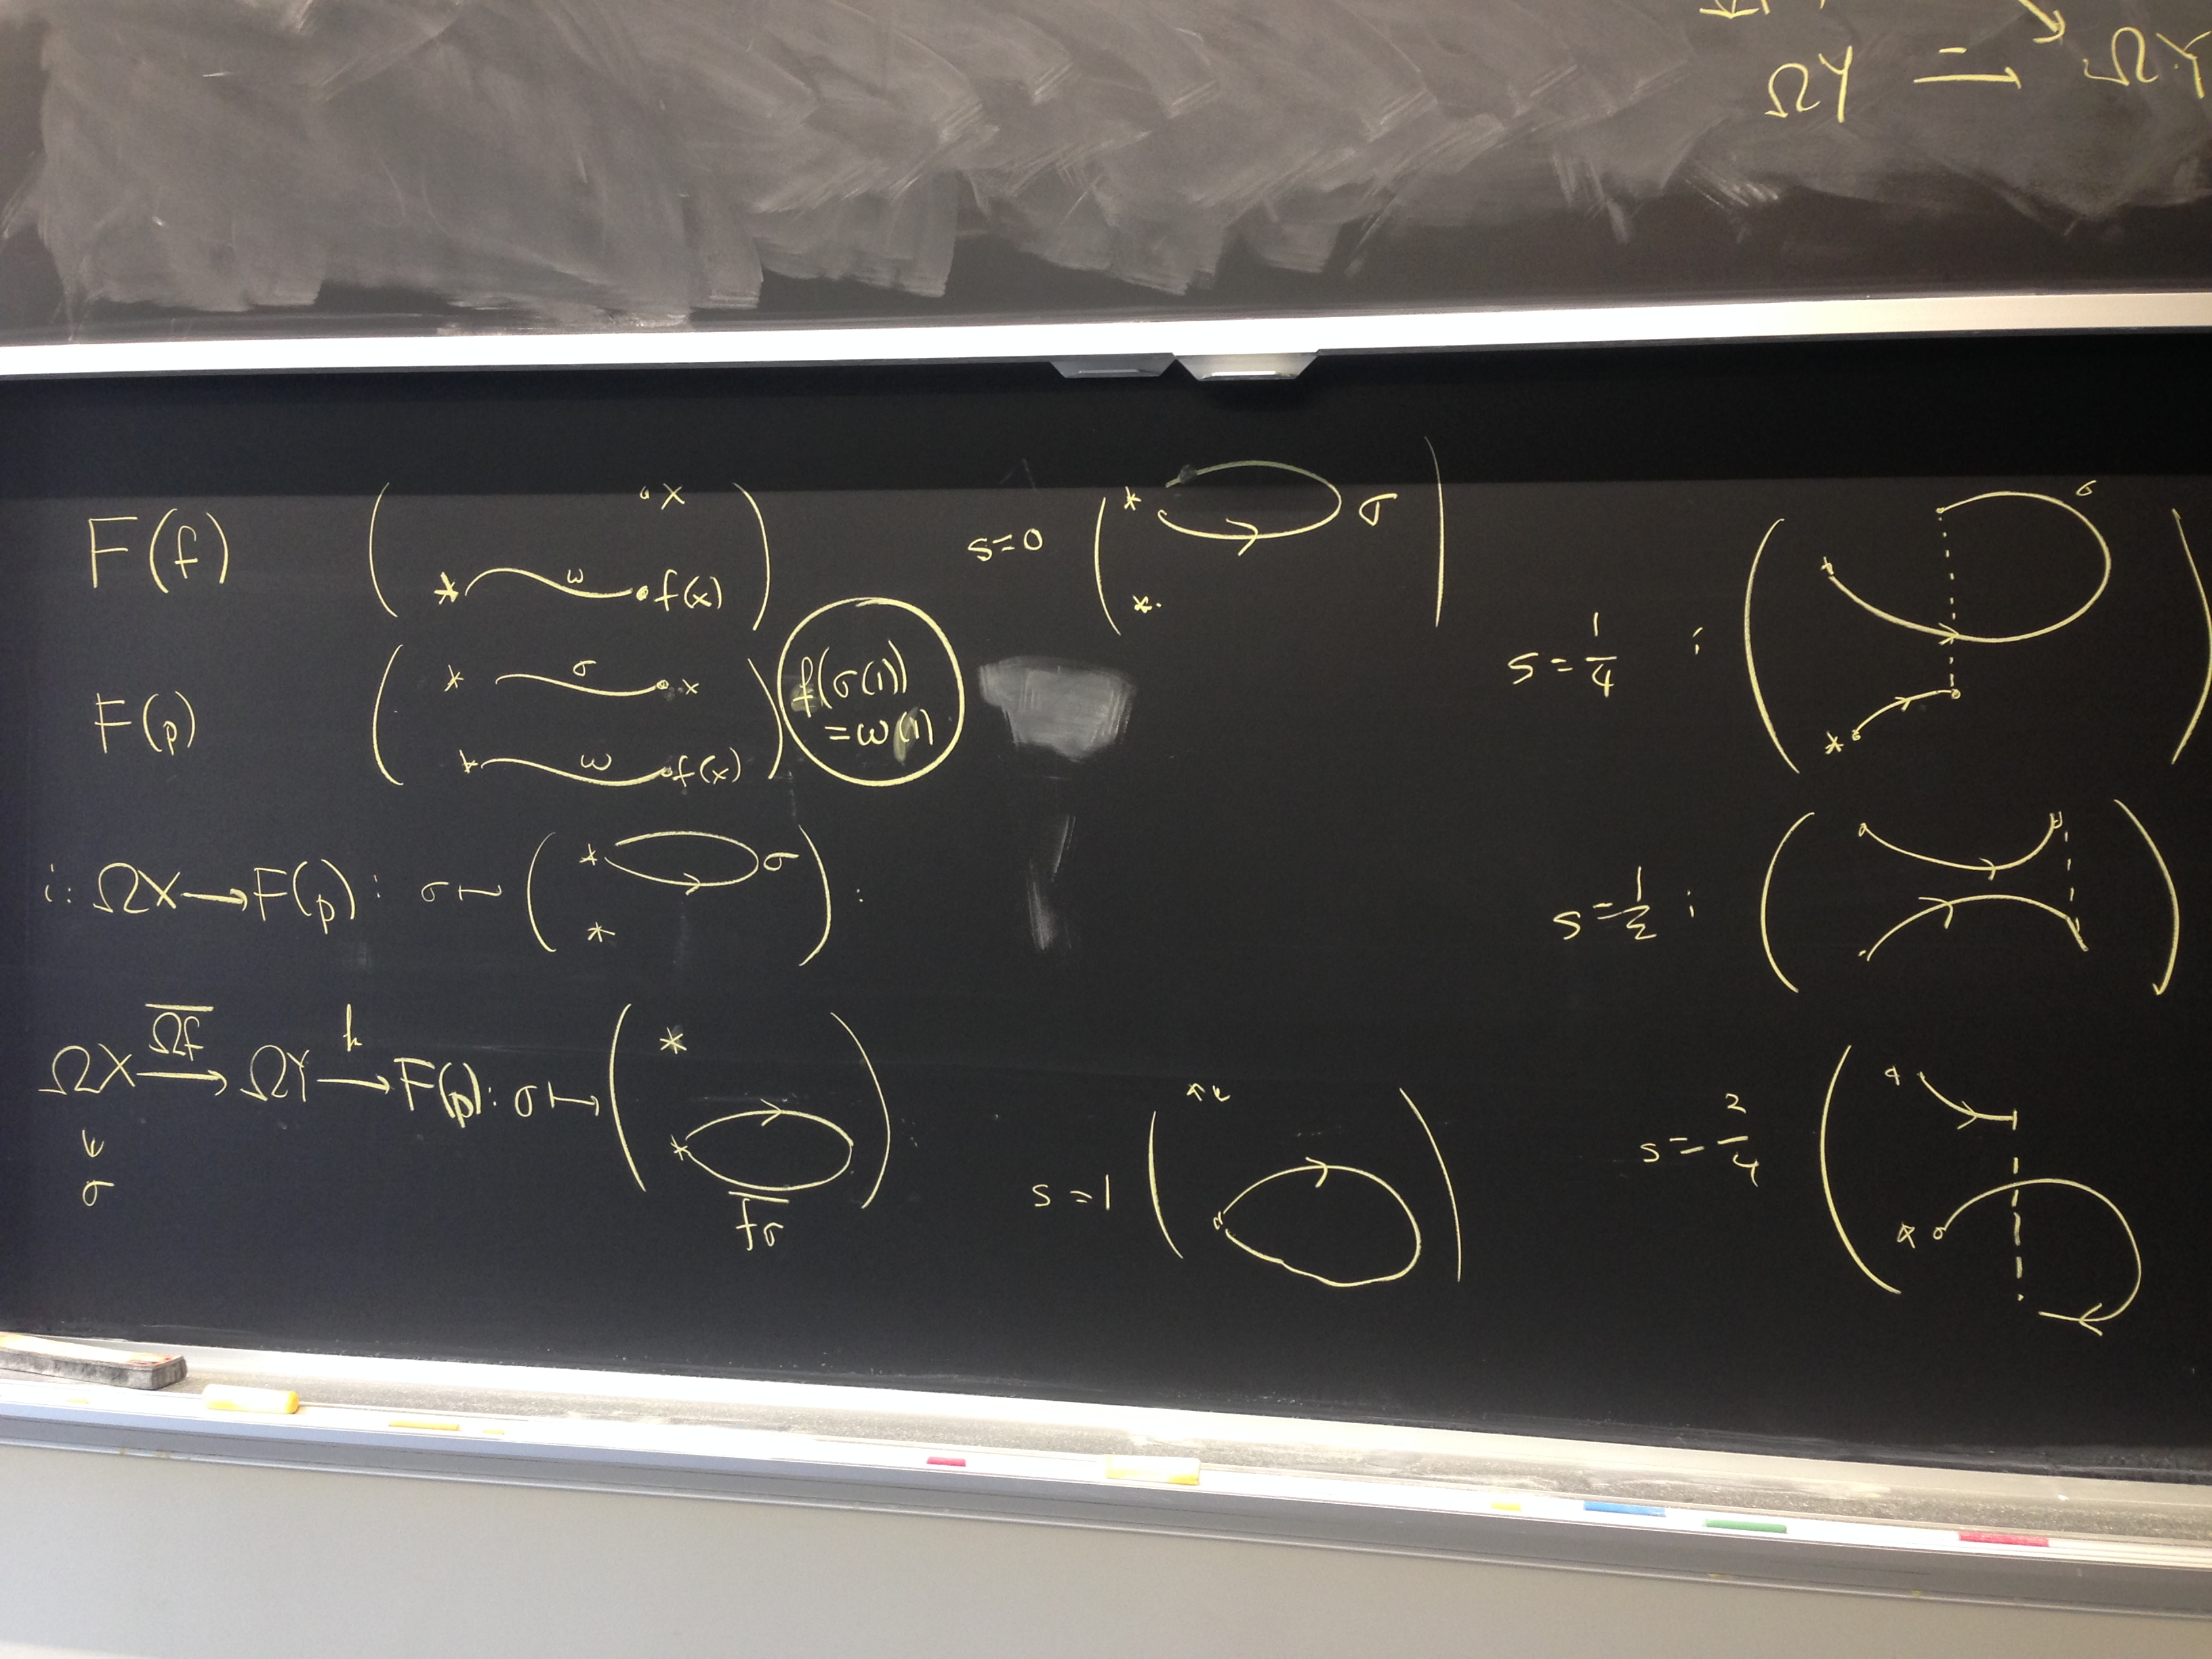
\includegraphics[width=\textwidth]{barratt-puppe}
\caption{A proof of this lemma.}
\end{figure}
\end{proof}
\begin{lemma}
    The following diagram commutes:
    \begin{equation*}
	\xymatrix{
	    & F(\overline{\Omega p_0})\ar@{=}[dd]\ar[dr] & \\
	    \Omega^2 Y\ar[ur]^{i(\Omega p_0)}\ar[dr]_{\overline{\Omega i(p_0)}} & & \Omega X\\
	    & \Omega Fp_0\ar[ur]_{\overline{\Omega p_1}} & 
	    }
    \end{equation*}
\end{lemma}
What is the map $F\overline{\Omega p_0}\to \Omega X$?? We spent some time figuring this out. But you can now apply $[W,-]_\ast$ to the following diagram to get a long exact sequence:
\begin{equation*}
    \xymatrix{
	\cdots\ar[r] & Fp_4\ar[r] & Fp_3 \ar[r] & Fp_2\ar[r] & Fp_1\ar[r]^{p_2} & Ff\ar[r]^{p_1} & X\ar[r]^{f} & Y\\
    \cdots\ar[r] & \Omega Fp_1\ar[r]|{\overline{\Omega p_2}}\ar[u]_{\simeq} & \Omega Fp_0\ar[u]_{\simeq}\ar[ur]|{i(p_2)}\ar[r]|{\overline{\Omega p}} & \Omega X\ar[r]|{\overline{\Omega f}}\ar[u]_{\simeq}\ar[ur]|{i(p_1)} & \Omega Y\ar[u]_\simeq \ar[ur]|{i(p_0)} & &\\
	\Omega^2 X\ar[u]_{\simeq}\ar[r]_{\Omega f} & \Omega Y\ar[u]_{\simeq}\ar[ur]_{\overline{\Omega i(p_0)}} & & &
    }
\end{equation*}

For example, $S^0=\{\pm 1\}$. We get terms like $\pi_0(\Omega^n X)$, because $[S^0,X] = \pi_0 X$. What is $\pi_0(\Omega^n X)$? This is $[S^0,\Omega^n X]_\ast$. Is it clear to you that this is $[S^n,X]_\ast$?

Ok, well, $\Omega^2 X = (\Omega X)^{S^1}$. Because $(S^1)^{\wedge n} = S^n$. So we find that $(\Omega X)^{S^1} = (X^{S^1}_\ast)^{S^1}_\ast = X_\ast^{S^1\wedge S^1} = X_\ast^{S^2}$.

Well, $\Omega X$ is a homotopy group by concatenation. It's a group, but where the axioms hold up to homotopy. It's a group in the homotopy category. Therefore, $\pi_0 \Omega X$ is a group! It's exactly $\pi_1 X$, which you know to be a group. And then, there's this other thing that happens.

You can think of $\pi_n(X) = [S^n,X]_\ast$ as $[(D^n,S^{n-1}),(X,\ast)] = [(I^n,\partial I^n),(X,\ast)]$. If I take $n=2$, for example, how do I take the product of $\alpha,\beta\in \pi_2(X)$? You just literally put them together (when you think of $\pi_2(X) = [(I^2,\partial I^2),(X,\ast)]$. You can play this game; up to homotopy, you can shrink $\alpha$ and $\beta$ to make them as small I want, and then reverse their position and expand them again\footnote{This probably makes no sense without a picture}\todo{Add a picture}. Thus $\pi_2(X)$ is an abelian group.

Thus, when you apply $\pi_0$ to our sequence $\cdots\to\Omega^2 X\to\Omega^2 Y\to \Omega Fp_0\to \Omega X\to \Omega Y\to Fp_0\to \Omega X\to \Omega Y$, you get an exact sequence (of groups when the homotopy groups are $>0$, and of pointed sets when you have $\pi_0$):
$$\cdots\to \pi_2 X\to \pi_2 Y\to \pi_1 Ff\to \pi_1 X\to\pi_1 Y\to\pi_0 Ff\to\pi_0 X\to \pi_0 X$$
\section{Relative homotopy, $\pi_1$ action}
Pset 2 has question 8; there's still one more to go. Hood has office hours today 12 -- 1 in 2-390, and I have office hours today tomorrow 4-5 in 2-478.
\subsection{Spheres and homotopy groups}
Let's talk about spheres, first of all. The $n$-sphere is $S^n=I^n/\partial I^n$. Agreed? It's a standard choice. By the way, $S^1 = I/0\sim 1$. What about $S^0$? This is $\ast/\emptyset = \ast_+$. This is the usual way to think of the zero sphere. The point that you just added is the basepoint.

We have this looping thing going on; we know that $\Omega X$ (I'm always working in $\Top_\ast$ these days) is $X^{S^1}_\ast$. Thus the adjunction says that $\Top_\ast(W,\Omega X) = \Top_\ast(S^1\wedge W,X)$.
\begin{definition}
    The \emph{reduced suspension} $\Sigma W$ is $S^1\wedge W$.
\end{definition}
If I have $A\subseteq X$, then $X/A\wedge Y/B = (X\times Y)/((A\times Y)\cup_{A\times B}(X\times B))$. Thus $\Sigma X = S^1\wedge X$ is $I\times X/(\partial I \times X\cup I\times \ast)$. I collapse the top and bottom of a cylinder to a point, and also the line along a basepoint gets collapsed.

Similarly, $\Sigma^n X$ is the left adjoint of the $n$-fold loop space. Hence $\Sigma^n X = (S^1)^{\wedge n}\wedge X$. What is $S^1\wedge S^n$? This is $I/\partial I\wedge I^n\wedge \partial I^n = (I\times I^n)/(\partial I\times I^n\cup I\times \partial I^n)$. This denominator is exactly $\partial I^{n+1}$; hence $S^1\wedge S^n\simeq S^{1+n}$. In fact, $S^k\wedge S^n\simeq S^{k+n}$.
\begin{definition}
    The $n$th homotopy group of $X$ is $\pi_n X = \pi_0(\Omega^n X)$.
\end{definition}
This is $[S^0,\Omega^n X]_\ast = [S^n, X]_\ast = [(I^n,\partial I^n),(X,\ast)]$.
\subsection{The homotopy category}
We have the \emph{homotopy category of spaces} $\Ho(\Top)$ whose objects are spaces and whose mapping spaces are $\pi_0$ of mapping spaces. I have to check that if $f_0,f_1:X\to Y$ and $g:Y\to Z$, then $gf_0\simeq gf_1$. Of course, it is, just by composing with $g$. Similarly $f_0h\simeq f_1h$. This guarantees that you can define composition of maps in $\Ho(\Top)$. I can also think about $\Ho(\Top_\ast)$, with pointed homotopies. A lot of what we've been doing has been taking place in $\Ho(\Top_\ast)$.

Fix $W$. We need to check that $X\mapsto X^W_\ast$ is a homotopy functor. It defines a functor $\Top_\ast\to\Top_\ast$. Namely, I want to complete:
\begin{equation*}
    \xymatrix{
	\Top_\ast\ar[d]\ar[r]^{X\mapsto X^W_\ast} & \Top_\ast\ar[d]\\
	\Ho(\Top_\ast)\ar@{-->}[r] & \Ho(\Top_\ast)
    }
\end{equation*}
So I'd better check that if I have a homotopy $f_0\sim f_1:X\to Y$. Is that a map $I\wedge X\to Y$? This really tells you that there's a nullhomotopy if the basepoint of $I$ is one of the endpoints. I really want to consider $I\times X/I\times\ast$. Aha, but this is just $I_+\wedge X$. So a homotopy $f_0\sim f_1:X\to Y$ is a map $I_+\wedge X\to Y$.

Suppose I have a homotopy like this; then I get $(I_+\wedge X)^W\to Y^W_\ast$. I wanted $I_+\wedge X^W_\ast\to Y^W_\ast$, so that's not quite what I wanted. I can get this if I can construct a map $I_+\wedge X^W_\ast\to (I_+\wedge X)^W_\ast$. In fact, I want to construct $A\wedge X^W_\ast\to (A\wedge X)^W_\ast$. One thing I can do is $A\wedge X^W_\ast\to A^W_\ast\wedge X^W_\ast$ by sending $a\mapsto c_a$, and then the exponential law gives a homotop $A^W_\ast\wedge X^W_\ast\to (A\wedge X)^W_\ast$. This gives me a map $I_+\wedge X^W_\ast\to (I_+\wedge X)^W_\ast\to Y^W_\ast$ making $X\mapsto X^W_\ast$ a homotopy functor. In particular, $\Omega^n$ is a homotopy functor.

Let's continue with this homotopical localization of things.
\begin{definition}
    A fiber sequence in $\Ho(\Top_\ast)$ is a composite $X\to Y\to Z$ that is isomorphic in $\Ho(\Top_\ast)$ to some $Ff\xrightarrow{p} E\xrightarrow{f}B$. Namely we want some (possibly zig-zag of) maps that are homotopy equivalences:
    \begin{equation*}
	\xymatrix{
	    X\ar[r]\ar[d] & Y\ar[r]\ar[d] & Z\ar[d]\\
	    Ff\ar[r]_p & E\ar[r]_f & B
	    }
    \end{equation*}
\end{definition}
We've seen examples in our elaborate story. Recall our diagram:
\begin{equation*}
    \xymatrix{
	\cdots\ar[r] & Fp_4\ar[r] & Fp_3 \ar[r] & Fp_2\ar[r] & Fp_1\ar[r]^{p_2} & Ff\ar[r]^{p_1} & X\ar[r]^{f} & Y\\
    \cdots\ar[r] & \Omega Fp_1\ar[r]|{\overline{\Omega p_2}}\ar[u]_{\simeq} & \Omega Fp_0\ar[u]_{\simeq}\ar[ur]|{i(p_2)}\ar[r]|{\overline{\Omega p}} & \Omega X\ar[r]|{\overline{\Omega f}}\ar[u]_{\simeq}\ar[ur]|{i(p_1)} & \Omega Y\ar[u]_\simeq \ar[ur]|{i(p_0)} & &\\
	\Omega^2 X\ar[u]_{\simeq}\ar[r]_{\Omega f} & \Omega Y\ar[u]_{\simeq}\ar[ur]_{\overline{\Omega i(p_0)}} & & &
    }
\end{equation*}
So look, $Ff\to X\to Y$ is a fiber sequence. And $\Omega Y\to F\xrightarrow{p}X$ is another fiber sequence because it's isomorphic to $Fp\to F\to X$ in $\Ho(\Top_\ast)$. I also have $\Omega X\xrightarrow{\overline{\Omega f}}\Omega Y\to F$ is another fiber sequence. This means that $\Omega X\xrightarrow{\Omega f}\Omega Y\to F$ is another fiber sequence because these two fiber sequences differ by an automorphism of $\Omega X$ because in general, if $A^\prime\xrightarrow{\sim} A$ and $A\to B\to C$ is a fiber sequence, so is $A^\prime\xrightarrow{\sim} A\to B\to C$.

I can apply $\Omega$ again, so I get $\Omega F\xrightarrow{\Omega p} \Omega X\xrightarrow{\Omega f} \Omega Y$. I claim this is a fiber sequence, because this is a loop of a fiber sequence, and taking loops takes fiber sequences to fiber sequences. This is called the \emph{Barratt-Puppe sequence}. I carefully explained that this makes some sense, because it firstly makes sense to ask that $\Omega$ is a homotopy functor. I haven't said this yet. So in particular:
\begin{enumerate}
    \item $\Omega$ takes fiber sequences to fiber sequences.
    \item $\Omega Ff\simeq F\Omega f$. Check this!
\end{enumerate}
You can now \emph{loop back} to get $\Omega^2 Y\xrightarrow{\Omega i} \Omega F\xrightarrow{\Omega p}\Omega X$. This is an unstable version of a triangulated category. It wants to be a triangulated category, but it isn't.
\begin{remark}
    If $f:X\to Y$, I can form $Ff$. I might have a homotopy commuting diagram like:
    \begin{equation*}
	\xymatrix{
	    \Omega Y\ar[d]_{\Omega g}\ar[r] & Ff\ar@{-->}[d]\ar[r] & X\ar[d]_{h}\ar[r]^f & Y\ar[d]^g\\
	    \Omega Y^\prime\ar[r] & Ff^\prime\ar[r] & X^\prime\ar[r]_{f^\prime} & Y
	    }
    \end{equation*}
    The dotted map exists, but \emph{this map depends on the homotopy} $f^\prime h\simeq gf$. That's an important subtlety.
\end{remark}
\subsection{Lexseq of a fiber sequence}
Applying $\pi_0 = [S^0,-]_\ast$ to the Barratt-Puppe sequence gives a lexseq:
\begin{equation*}
    \xymatrix{
	& \cdots\ar[r] & \pi_2 Y\ar[dll]\\
	\pi_1 F\ar[r] & \pi_1 X\ar[r] & \pi_1 Y\ar[dll]\\
	\pi_0 F\ar[r] & \pi_0 X\ar[r] & \pi_1 X
    }
\end{equation*}
of pointed sets. But this is even better, ,because $\Omega X$ is a group object in $\Ho(\Top_\ast)$.
\begin{remark}
    $\Ho(\Top)$ and $\Ho(\Top_\ast)$ has products and coproducts, but very few other limits or colimits. So as a category, it is \emph{horrible}.
\end{remark}
I showed you an argument that $\Omega^2 X$ is an \emph{abelian} group object, i.e., multiplication is commutative up to homotopy. Thus $\pi_1$ is a group and $\pi_k$ is an abelian group for $k\geq 2$; hence in our diagram above, all maps (except on $\pi_0$) are group homomorphisms!

What if $X\to Y$ is the inclusion $i:A\hookrightarrow X$ of a subspace? Then $Fi=\{(a,\omega)\in A\times X^I_\ast|\omega(1) = a\}$. This is just the collection of all paths that begin at $\ast\in A$ and ends in $A$.
\begin{definition}
    $\pi_n(X,A,\ast) = \pi_n(X,A)$ is $\pi_{n-1}Fi = [(I^n,\partial I^n,(\partial I^n\times I)\cup (I^{n-1}\times 0)),(X,A,\ast)]$.
\end{definition}
Inside $I^n$ is $\partial I^n$, and also including in it is $\partial I^n\times I\cup I^{n-1}\times 0$. Then you can check that $\pi_{n-1}Fi = [(I^n,\partial I^n,(\partial I^n\times I)\cup (I^{n-1}\times 0)),(X,A,\ast)]$. In this case, you have a lexseq: 
\begin{equation*}
    \xymatrix{
	& \cdots\ar[r] & \pi_2 (X,a)\ar[dll]\\
	\pi_1 A\ar[r] & \pi_1 X\ar[r] & \pi_1 (X,A)\ar[dll]\\
	\pi_0 A\ar[r] & \pi_0 X\ar[r] & 
    }
\end{equation*}
\section{Action of $\pi_1$, simple spaces, and the Hurewicz theorem}
Recall that $\pi_n(X,A,\ast) = [(I^n,\partial I^n,\partial I^{n-1}\times I\cup I^{n-1}\times 0),(X,A,\ast)]$. You have a lexseq of the form:
\begin{equation*}
    \xymatrix{
	& \cdots\ar[r] & \pi_2 (X,a)\ar[dll]\\
	\pi_1 A\ar[r] & \pi_1 X\ar[r] & \pi_1 (X,A)\ar[dll]\\
	\pi_0 A\ar[r] & \pi_0 X\ar[r] & 
    }
\end{equation*}
This looks very similar to the lexseq for homology. How does this actually relate?
\begin{lemma}[Excision]
    If $A\subseteq X$ is a cofibration, then there is an isomorphism $H_\ast(X,A)\xrightarrow{\simeq}\widetilde{H}_\ast(X/A)$. Under this hypothesis, $X/A\simeq\text{Mapping cone of }i:A\to X$. The mapping cone is the dual to the homotopy fiber, i.e., the homotopy quotient, which is defined by the pushout:
    \begin{equation*}
	\xymatrix{
	    A\ar[r]^i\ar[d]^{in_1} & X\ar[d]\\
	    CA\ar[r] & X\cup_A CA
	    }
    \end{equation*}
    where $CA$ is the cone on $A$ defined as $CA = A\times I/A\times 0$ (this is a contractible space).
\end{lemma}
This is dual to saying that $Ff\simeq f^{-1}(\ast)$ if $f$ is a fibration.

But $\pi_\ast(X,A)$ is definitely not $\pi_\ast(X/A)$! For example, $S^1\to D^2\to S^2$ is a cofibration sequence, but $\pi_\ast S^1$ is just $\Z$ in dimension $1$. We don't know the homotopy groups of $S^2$, though. In fact:
\begin{theorem}[Now]
    If $X$ is a simply connected finite complex, and $X\not\simeq \ast$, then we do not know $\pi_\ast(X)$. And we'll probably never be able to know them.
\end{theorem}
These groups \emph{are} computable (a theorem by Edgar Brown), but it's super-exponential. This is discouraging. We'll never know what, eg., $\pi_{10000}(S^2)$ is.

Anyway, I said there was $\partial:\pi_n(X,A,\ast)\to \pi_{n-1}(A,\ast)$. How does this look? Well you just look at the restriction of $I^n\to X$ to $1\times I^{n-1}\to A$. And the composite $\pi_n(X,A,\ast)\xrightarrow{\partial}\pi_{n-1}(A,\ast)\to \pi_{n-1}(X,\ast)$ is trivial by definition!
\subsection{$\pi_1$-action}
There's a little more structure about this sequence. That's the following thing: $\pi_1(X)$ acts on $\pi_n(X)$ from the left by group homomorphisms. There was a picture, but I didn't understand it. Let me write this out (as I understand it). Suppose $x,y\in X$, and let $\omega:I\to X$ with $\omega(0) = x$ and $\omega(1) = y$. Then we have a map $f_\omega:\pi_n(X,x)\to \pi_n(X,y)$, so $\pi_1(X,\ast)$ acts on $\pi_n(X,\ast)$.

When $n=1$, $\pi_1(X)$ acts by conjugation. In fact, $\pi_1(A)$ acts on $\pi_n(X,A,\ast)$ as well. It then follows that all maps in the lexseq are equivariant for this action of $\pi_1(A)$. We also have the Peiffer identity:
\begin{prop}[Peiffer identity]
    let $\alpha,\beta\in \pi_2(X,A)$. Then $(\partial \alpha)\cdot\beta = \alpha\beta\alpha^{-1}$.
\end{prop}
For example, if $j:\pi_2(X)\to \pi_2(X,A)$, and $\alpha = j(\gamma)$, $\partial\alpha = 1$: $\img(k)\subseteq\coker \pi_2(X,A)$. (I did not follow this)

\begin{definition}
    $X$ is simply connected if it's path connected and $\pi_1(X,\ast) = 1$.
\end{definition}
Sometimes you have nontrivial $\pi_1$, and so:
\begin{definition}
    $X$ is \emph{simple} if it is path-connected and $\pi_1(X)$ acts trivially on $\pi_n(X)$ for $n\geq 1$.
\end{definition}
(In particular, $\pi_1(X)$ is abelian.) What does being simple do for you?
\begin{itemize}
    \item Being simple is independent of the choice of basepoint. If $\omega:x\to x^\prime$, then $\omega_\sharp:\pi_n(X,x)\to \pi_n(X,x^\prime)$ is a group isomorphism. I have $\pi_1(X,x)$ acting on $\pi_n(X,x)$ and $\pi_1(X,x^\prime)$ acting on $\pi_n(X,x^\prime)$. These actions are compatible, and if $\pi_1(X,x)$ acts trivially then so does $\pi_1(X,x^\prime)$.
    \item Say $X$ is path-connected. Then there's a map $\pi_n(X,\ast)\to [S^n,X]$. It's pretty obvious that this map is surjective because I can always choose a basepoint in $X$ as the image of a basepoint in $S^n$. Thus you'd expect a factorization:
	\begin{equation*}
	    \xymatrix{
		\pi_n(X,\ast)\ar@{->>}[r]\ar[dr] & [S^n,X]\\
		& \pi_1(X,\ast)\backslash \pi_n(X,\ast)\ar[u]_{\cong,\text{homework}}
		}
	\end{equation*}
	If $X$ is simple, then $\pi_1(X,\ast)\backslash \pi_n(X,\ast)$ is trivial, and so $\pi_n(X,\ast)\cong [S^n,X]$ that's independent of the basepoint. I.e., these groups are canonically the same, i.e., two paths $\omega,\omega^\prime:x\to y$ give the same map $\omega_\sharp = \omega^\prime_\sharp:\pi_n(X,x)\to \pi_n(X,y)$.
\end{itemize}
\subsection{Hurewicz theorem}
I talked about homotopy, and I talked about homology. Now it's time to compare the two. This is the story of the Hurewicz theorem. You should think of homology of being computable, while homotopy is a big mystery.
\begin{definition}
The Hurewicz map is a map $h:\pi_n(X,\ast)\to H_n(X)$, where $X$ is a path connected space. How does this map go? An element in $\pi_n(X,\ast)$ is represented by $\alpha:S^n\to X$. Pick a generator $\sigma:H_n(S^n)$; then $\alpha_\ast(\sigma)\in H_n(X)$.
\end{definition}
This is a homomorphism, as I'll show in a bit.

What happens when $n=0$? What map $\pi_0(X)\to H_0(X)$ do we have? A point is like a $0$-cycle, and that's the map! In fact, we have an isomorphism $H_0(X)\simeq \Z[\pi_0(X)]$. This is an example of the Hurewicz theorem.

How about $n=1$? Now, we have $h:\pi_1(X,\ast)\to H_1(X)$. This factors as $\pi_1(X,\ast)\to \pi_1(X,\ast)^{ab}\to H_1(X)$. And the Hurewicz theorem says that $\pi_1(X,\ast)^{ab}\xrightarrow{\simeq} H_1(X)$. I'm not going to prove this; it's not very hard but it's annoying. It's pretty clear why it's true: for example, it's onto. $1$-cycles just look like a bunch of circles, so just concatenate loops from the basepoint to these $1$-cycles.

Let me show you that the Hurewicz map is a homomorphism. Before that, here's the Hurewicz theorem.
\begin{theorem}[Hurewicz]
    Suppose $\pi_i(X) = 0$ for $i<n$ where $n\geq 2$. Then $\pi_n(X)\xrightarrow{\simeq}H_n(X)$.
\end{theorem}
We can't compute homotopy in general, but we can at least make a start.

OK, why is $h$ a homomorphism? Let $\alpha,\beta:S^n\to X$ be pointed maps. What is the product in $\pi_n(X)$? It's just the composite:
$$\alpha\beta:S^n\xrightarrow{\delta\text{, pinching along the equator}} S^n\vee S^n\xrightarrow{\beta\vee\alpha}X\vee X\xrightarrow{\nabla\text{, the fold map}}X$$
where $\nabla:X\vee X\to X$ is defined by:
\begin{equation*}
    \xymatrix{
	X\ar[dr]^1\ar[d] & \\
	X\vee X\ar[r]|\nabla & X\\
	X\ar[u]\ar[ur]_1 & 
    }
\end{equation*}
We have two inclusions $in_1,in_2$ of $S^n$ to $S^n\vee S^n$. Now, we have:
$$\sigma\mapsto {in_1}_\ast\sigma + {in_2}_\ast\sigma\mapsto {in_1}_\ast h(\alpha) + {in_2}_\ast h(\beta)\mapsto h(\alpha) + h(\beta)$$
As desired. It's possible to give an elementary proof of Hurewicz's theorem. But I'll prove this as a consequence of the Serre spectral sequence, which gives a more genral theorem. It'll be an inductive proof that'll use Poincare's result.

One more thing to say is that $\pi_i(S^n) = 0$ if $i<n$. I won't prove this, but it's also kind of obvious, isn't it? By Hurewicz, it follows that $\pi_n(S^n)\simeq H_n(S^n)\simeq \Z$. We actually have one more example: $\pi_3(S^2)\simeq \Z$ generated by the Hopf fibration $S^3\to S^2$. It's not obvious that this isn't nullhomotopic, but it's true. But now, for example, I can suspend $\eta$ (the Hopf fibration) and get $\eta\circ\Sigma\eta$. We thought for a long time that there were the only things we could compute in $\pi_\ast S^n$; but this is not true! It's a lot more chaotic.
\section{Some examples; CW complexes}
\subsection{Examples}
\begin{enumerate}
    \item Let $E\to B$ be a covering space with $E$ and $B$ connected. The fibers are discrete, so they don't have any higher homotopy. There's only $\pi_0$. The lexseq says that $\pi_n(E)\to \pi_n(B)$ is an isomorphism for $n>1$, and $\pi_1(E)\hookrightarrow \pi_1(B)$, and the subgroup $\pi_1(E)$ classifies the covering space. In general, we know that $\Omega B$ acts on the homotopy fiber $F$. Because $F$ here is discrete, this action factors through $\pi_0(\Omega B)\simeq \pi_1(B)$.

	In particular, $\pi_q(S^n)\simeq \pi_q(\RP^n)$ for $q>1$. Of course, $\pi_1(\RP^n)\simeq \Z/2\Z$. This creates a ton of homology in $\RP^n$ that's not present in the homology of $S^n$. Here's a piece of language.

	\begin{definition}
	    A space is \emph{$n$-connected} if $\pi_i(X) = 0$ for $i\leq n$.
	\end{definition}
	This is not a nonsense definition, although it seems like we need to pick a basepoint -- but $0$-connected means path connected, so we're good. For instance, $1$-connected means simply connected.

	Suppose $E\to B$ is a covering space where $E$ is $n$-connected. Then $\pi_1(B)$ determines the homology $H_i(B)$ in dimensions $i<n$. In particular, $H_i(B) = H_i(\pi_1(B))$, which is the group homology. This is due to Heinz Hopf.
    \item What's a nontrivial action of $\pi_1$ on higher homotopy? For example, $\pi_1$ acting on $\pi_2$. Consider the space $S^1\vee S^2$. What does the universal cover $E$ look like? This just $\RR$, where at every integer point I put a $2$-sphere $S^2$. The universal cover is simply connected, so Hurewicz says that $\pi_2(E)\simeq H_2(E)$. Up to homotopy type, I can collapse the line to a point, so I get a countable bouquet of $2$-spheres. Thus $\pi_2(E)\simeq H_2(E) = \bigoplus^\infty\Z$. But I can say more!

	There's an action of $\pi_1(S^1\vee S^2)$ on $E$. Certainly $\pi_1(S^1\vee S^2) = \Z$. There's an induced action on $E$. All the action does is shift the $2$-spheres on the integer points of $\RR$ (on $E$) to the right by $1$. Thus $\bigoplus^\infty\Z=\Z[\pi_1(B)]$ as a $\Z[\pi_1(B)]$-module (i.e., as a $\Z[\Z]$-module). That's actually the same action of $\pi_1(E)$ on $\pi_2(E)$.	This tells something horrifying. $S^1\vee S^2$ is a very simple $3$-complex, but its homotopy is huge.
    \item $\pi_\ast(X)=?$. Recall our Hopf fibration $S^1\to S^3\to S^2$. This gives a lexseq on homotopy groups. Thus I get $\pi_i(S^3)\xrightarrow{\simeq}\pi_i(S^2)$ for $i>2$ given by $\alpha\mapsto\eta\alpha$. Of course, $\pi_2(S^2) = \Z$. The higher homotopy groups of $S^2$ are exactly the same as the higher homotopy groups of $S^3$! In particular, $\pi_3(S^3)=\Z$ by Hurewicz, so $\pi_3(S^2)\simeq \Z$ generated by $\eta$. There are some low-dimensional calculations that you can make like this.

	Here's another way of thinking of the Hopf fibration. Think of $S^3 = SU(2)$. Then there's the subgroup of $\begin{pmatrix}\lambda & \\ & \lambda^{-1}\end{pmatrix}$, which is $S^1$. This acts on $S^3$ by translation, and the orbit space is $S^2$.

	We'll show later that $\pi_{4n-1}(S^{2n})\otimes\QQ\simeq \QQ$. Other than $\pi_n(S^n)$, a theorem of Serre says that these are the only non-torsion homotopy groups of spheres.
\end{enumerate}
\subsection{Bringing you up-to-speed on CW-complexes}
I want to study a fairly rich example of CW-complexes.
\begin{definition}
    A \emph{relative} CW-complex is a pair $(X,A)$ together with a fitration $A=X_{-1}\subseteq X_0\subseteq X_1\subseteq\cdots\subseteq X$, such that for all $n$, I can build $X_n$ as the pushout:
    $$
    \xymatrix{
	\coprod_{\alpha\in \Sigma_n}S^{n-1}\ar[r]\ar[d]_{\text{attaching maps}} & \coprod_{\alpha\in \Sigma_n}D^n\ar[d]^{\text{characteristic maps}}\\
	X_{n-1}\ar[r] & X_n
    }
    $$
    ($X_n$ is called the $n$-skeleton), and $X=\varinjlim X_n$.
\end{definition}
If $A=\emptyset$, it's not relative anymore -- it's just a CW-complex. (Here $S^{-1} = \emptyset$.) Often, $X$ will be a CW-complex, and $A$ will be a subcomplex.
\begin{enumerate}
    \item If $A$ is Hausdorff, then so is $X$. Actually, last semester I discovered a proof of this in Hatcher.
    \item $A=\emptyset$: then $X$ is compactly generated. This is one of the reasons I wanted to define compactly generated spaces.
    \item If $X$ and $Y$ are both CW-complexes. Then define $(X\times^k Y)_n = \bigcup_{i+j = n}X_i\times Y_j$. This gives a CW-structure on the product $X\times^k Y$.
    \item Any closed smooth manifold admits a CW-structure. 
\end{enumerate}
The fun example is $\CP^n$.
\begin{example}
    $\CP^n$ is a CW-complex, with skeleta $\CP^0\subseteq\CP^1\subseteq\cdots\subseteq \CP^n$. The assertion is that there's a pushout diagram:
    \begin{equation*}
	\xymatrix{
	    \coprod S^{2n-1}\ar[r]\ar[d] & \coprod D^{2n}\ar[d]\\
	    \CP^{n-1}\ar[r] & \CP^n
	    }
    \end{equation*}
    Any complex line through the origin meets the hemisphere defined by $\begin{pmatrix}z_0\\\vdots\\z_n\end{pmatrix}$ with $||z||=1$ and $\Im(z_n) = 0$ and $\Re(z_n)\geq 0$. It meets this hemisphere (which is $D^{2n}$) at one point, unless it's on the equator, in which case we find that the pushout diagram is really:
    \begin{equation*}
	\xymatrix{
	    S^{2n-1}\ar[r]\ar[d] & D^{2n}\ar[d]\\
	    \CP^{n-1}\ar[r] & \CP^n
	    }
    \end{equation*}
\end{example}
I want to give you a more complicated example that's fun and that will come up later.
\begin{example}[Grassmannians]
    Let $V=\RR^n$ or $\cc^n$ or $\HH^n$. Let's suppose $V=\RR^n$ for now. Then $\Gra_k(\RR^n)$ is the collection of $k$-dimensional subspaces of $\RR^n$. One way to do this is by giving a $k\times n$ rank $k$ matrix. Here's some linear algebra.

    The span of rows of $A$ is the row space $V_A$. This is the span of the rows of the reduced reduced echelon form of $A$. An entry is a \emph{pivot} if its leftmost nonzero is in its row. A column is \emph{pivotal} if it contains a pivot. Any matrix is reduced echelon if the $i$th pivotal column is $e_i$.

    For instance, $\Gra_2(\RR^4)$ is as a set the disjoint union of:
    \begin{equation*}
	\begin{pmatrix}& 1 & \\ & & 1\end{pmatrix},\begin{pmatrix}&1&\ast\\&&1\end{pmatrix},\begin{pmatrix}1&\ast&\ast\\&&1\end{pmatrix},\begin{pmatrix}&1&\ast\\&1&\ast\end{pmatrix},\begin{pmatrix}1&\ast&\ast\\&1&\ast\end{pmatrix},\begin{pmatrix}1&\ast&\ast\\1&\ast&\ast\end{pmatrix}
    \end{equation*}
    So, define:
    \begin{definition}
	$\mathrm{sk}_j\Gra_k(\RR^n)$ is $\{V:\text{row ech rep with $\leq j$ free entries}\}$.
    \end{definition}
    The claim is that it's a CW-structure. See Milnor-Stasheff. They don't know it in 18.06, but they're constructing a CW-structure for the Grassmannian.
\end{example}
    The complex Grassmannian has cells in only even dimensions. We now know what the homology of the Grassmannian is, so we actually find Poincare duality if we count the number of cells in this case. (This is visible, for instance, in $\Gra_2(\RR^4)$). By the way, the top-dimensional cell tells us that $\dim\Gra_k(\RR^n) = k(n-k)$.
\section{Relative Hurewicz and J.~H.~C.~Whitehead}
I find what I'm talking about today very confusing, because there's this number, this $n$. I'm going to essentially read from my notes, because I'll get confused otherwise.
\begin{definition}
    Let $n\geq 0$. Say that $X$ is $(n-1)$-connected if for all $0\leq k\leq n$, and any $f:S^{k-1}\to X$ extends:
    \begin{equation*}
	\xymatrix{
	S^{k-1}\ar[d]\ar[r] & X\\
	D^k\ar@{-->}[ur] & 
	}
    \end{equation*}
\end{definition}
    Let's see what happens in low dimensions. When $n=0$, we know that $S^{-1} = \emptyset$, and $D^0 = \ast$. Saying that you're $(-1)$-connected is just saying that you're nonempty. If $n=1$, then this is saying that you're path connected, i.e., $0$-connected iff path connected. You can check that this is exactly the same as what we said before, using homotopy groups.

\begin{definition}
    Let $n\geq 0$. Say that $(X,A)$ is $n$-connected if for all $0\leq k\leq n$, there's a lift:
    \begin{equation*}
	\xymatrix{
	    (D^k,S^{k-1})\ar[r]^f\ar@{-->}[d] & (X,A)\\
	    (A,A)\ar[ur] & 
	    }
    \end{equation*}
    up to homotopy. In other words, you can homotope $f$ to a map with image in $A$, without moving $f|_{S^{k-1}}$.
\end{definition}
What does this mean for small values? When $n=0$, we find that $0$-connected means that $A$ meets every path component of $X$.

Equivalently, we can state:
    \begin{definition}
	$(X,A)$ is $n$-connected if:
	\begin{itemize}
	    \item $n=0$: then $\pi_0(A)\to \pi_0(X)$ surjects.
	    \item $n>0$: then $\pi_0(A)\xrightarrow{\simeq}\pi_0(X)$, and for all $a\in A$, $\pi_k(X,A,a) = 0$ for $1\leq k\leq n$. Equivalently, $\pi_0(A)\xrightarrow{\simeq}\pi_0(X)$ and $\pi_k(A,a)\to\pi_k(X,A)$ is an isomorphism for $1\leq k<n$ and is onto for $k=n$.
	\end{itemize}
    \end{definition}
    So ``$\pi_0(X,A) = 0$'' makes sense, because it means $\pi_0(A)\to \pi_0(X)$ surjects. I can't define $\pi_0(X,A)$, but you should think of it this way.

Let's try to write down what the relative Hurewicz theorem might be.
\subsection{Relative Hurewicz}
    Assume that $\pi_0(A) = \ast = \pi_0(X)$, and pick $a\in A$, which I won't bother about any more. We have:
    \begin{equation*}
	\xymatrix{
	    \cdots\ar[r] & \pi_2(X,A)\ar[r]\ar[d]^h & \pi_1(A)\ar[r]\ar[d]^h & \pi_1(X)\ar[r]\ar[d]^h & \pi_1(X,A)\ar[r]\ar[d]^h & \pi_0(A)\ar[r]\ar[d]^h & \pi_0(X)\ar[d]^h & \\
	    \cdots\ar[r] & H_2(X,A)\ar[r] & H_1(A)\ar[r] & H_1(X)\ar[r] & H_1(X,A)\ar[r] & H_0(A)\ar[r] & H_0(X)\ar[r] & H_0(X,A)
	    }
    \end{equation*}
How do we define the relative Hurewicz map? Let $\alpha\in \pi_n(X,A)$; then $\alpha:(D^n,S^{n-1})\to (X,A)$. So we pick a generator in $\Z\in H_n(D^n,S^{n-1})$, and send it to something in $H_n(X,A)$ under the induced $\alpha^\ast:H_n(D^n,S^{n-1})\to H_n(X,A)$.

Because $H_n(X,A)$ is abelian, we find that $\pi_1(A)$ acts trivially on $H_n(X,A)$, i.e., $h(\omega(\alpha)) = h(\alpha)$. Thus the relative Hurewicz map factors through $\pi_n^\dagger(X,A)$, which is $\pi_n(X,A)$ quotiented out by the normal subgroup generated by $(\omega\alpha)\alpha^{-1}$ where $\omega\in\pi_1(A)$ and $\alpha\in \pi_n(X,A)$. Thus you get a map $\pi_n^\dagger(X,A)\to H_n(X,A)$, that's more likely to be an isomorphism.
\begin{theorem}[Relative Hurewicz]
    Let $n\geq 1$. Assume $(X,A)$ is $n$-connected. Then $H_k(X,A) = 0$ for $0\leq k\leq n$, and $\pi_{n+1}^\dagger(X,A)\to H_{n+1}(X,A)$ is an isomorphism.
\end{theorem}
\begin{proof}
I won't prove this now; with any luck, we'll come back and prove this once we have the Serre spectral sequence in our toolkit.
\end{proof}
This is an extremely useful result. Now, that's it! That's all I wanted to say about the relative Hurewicz theorem. Let's apply this to get surprising results.
\subsection{J.~H.~C.~Whitehead theorems}
He was an interesting character. He raised pigs. He's interested in a continuous map $f:X\to Y$, and when that's an isomorphism in homology or homotopy, and relate them.
\begin{definition}
    Let $f:X\to Y$ and $n\geq 0$. Say that $f$ is an $n$-equivalence (some would say $n$-connected, but I won't say that here) if for every $\ast\in Y$, the homotopy fiber $F(f,\ast)$ is $(n-1)$-connected.
\end{definition}
A $0$-equivalence means that $\pi_0(X)$ surjects onto $\pi_0(Y)$. For $n>0$, this is saying that $\pi_0(X)\xrightarrow{\simeq}\pi_0(Y)$, and for every $\ast\in X$:
\begin{equation*}
    \pi_k(X,\ast)\to\pi_k(Y,f(\ast)) \text{ is }\begin{cases}
	\text{iso } & 1\leq k<n\\
	\text{epi, i.e., onto } & k = n
    \end{cases}
\end{equation*}
Would you like me to tell you about how to replace a map by a cofibration? Never mind -- this is the first problem! So, using the ``mapping cylinder'', we can always assume $f:X\hookrightarrow Y$, and then $f:X\to Y$ is an $n$-equivalence iff $(Y,X)$ is $n$-connected.
\begin{theorem}[J.~H.~C.~Whitehead 1]
    Suppose $n\geq 0$, and $f:X\to Y$ is $n$-connected. Then:
\begin{equation*}
H_k(X)\to H_k(Y) \text{ is }\begin{cases}
\text{iso } & 1\leq k<n\\
\text{epi, i.e., onto } & k = n
\end{cases}
\end{equation*}
\end{theorem}
\begin{proof}
    When $n=0$, because $\pi_0(X)\to \pi_0(Y)$ is surjective, $H_0(X)\simeq \Z[\pi_0(X)]\to \Z[\pi_0(Y)]\simeq H_0(Y)$ is surjective. The relative Hurewicz theorem gives the rest. Note that the relative Hurewicz dealt with $\pi_n^\dagger(X,A)$, but $\pi_n(X,A)\to\pi_n^\dagger(X,A)$ is surjective.
\end{proof}
Let me call out what happens when $n=\infty$.
\begin{definition}
    $f$ is a \emph{weak equivalence} (or an $\infty$-equivalence, to make it sound more impressive) if it's an $n$-equivalence for all $n$, i.e., it's a $\pi_\ast$-isomorphism.
\end{definition}
Putting everything together, we obtain:
\begin{corollary}
    A weak equivalence induces an isomorphism in integral homology.
\end{corollary}
Let's try to go in the other direction.

If $H_0(X)\to H_0(Y)$ surjects, then $\pi_0(X)\to \pi_0(Y)$ surjects also. Good start! Assume $X$ and $Y$ path connected. Suppose $H_1(X)$ surjects onto $H_1(Y)$. I'd like to know that $\pi_1(X)\to\pi_1(Y)$ surjects. It's hard to know this, though, because $H_1(X)$ is the abelianization. Let's give up and assume that $\pi_1(X)\to \pi_1(Y)$ is surjective.

Assume $\pi_1(X)$ surjects onto $\pi_1(Y)$. Assume $H_2(X)\to H_2(Y)$ surjects, and $H_1(X)\xrightarrow{\simeq}H_1(Y)$ surjects. We know that $H_2(Y,X) = 0$. On the level of the Hurewicz maps, I still don't know what to do because I only know about $\pi_2^\dagger$. What to do? Let's assume that $\pi_1(X)$ is trivial. That's a pretty radical assumption. It'd be enough to ask that $\pi_1(X)$ acts trivially on $\pi_2(Y,X)$. That's \emph{technically} what you want to assume. That's basically impossible to check. Anyway, if $\pi_1(X) = 0$, then $\pi_1(Y) = 0$. So $\pi_2(Y,X)$ is trivial, and we can go up the ladder.
\begin{theorem}[J.~H.~C.~Whitehead 2]
    Let $n\geq 2$. Assume that $\pi_1(X) = 0 = \pi_1(Y)$, and I have $f:X\to Y$ such that:
\begin{equation*}
H_k(X)\to H_k(Y) \text{ is }\begin{cases}
\text{iso } & 1\leq k<n\\
\text{epi, i.e., onto } & k = n
\end{cases}
\end{equation*}
then $f$ is an $n$-equivalence.
\end{theorem}
\begin{corollary}
    Let $X$ and $Y$ be simply-connected. If $f$ induces an isomorphism in homology, then it's a weak equivalence.
\end{corollary}
That's an \emph{incredibly} useful theorem, because we can actually compute homology! Let's complete this with a further theorem we'll prove on Wednesday.
\begin{theorem}
    If $Y$ is a CW-complex, a weak equivalence $f:X\to Y$ is in fact a homotopy equivalence!
\end{theorem}
\section{Cellular approximation, cellular homology, obstruction theory}
pset 3 is up in part. Today I'm going to tell you how to think about CW-complexes and work with them, and I won't give a lot of details. Some good sources are lecture notes by Davis-Kirk, and a beautiful book by Glen Bredon, as well as Hatcher.
\subsection{Cellular approximation}
\begin{theorem}
    Let $X$ and $Y$ be CW-complexes and $A\subseteq X$ a subcomplex. Let $f:X\to Y$ be a continuous map, and that $f|_{A}$ is skeletal\footnote{Some people would say cellular.}, i.e., $f(\Sigma_n)\subseteq Y_n$. It might not take cells in $A$ to cells in $Y$, but it takes $n$-skeleta to $n$-skeleta. Then $f$ is homotopic to some other $f^\prime:X\to Y$ relative to $A$ with $f^\prime$ skeletal on all of $X$.
\end{theorem}
This is kind of amazing.
\begin{lemma}[Key lemma]
    Any $(D^n,S^{n-1})\to (Y,Y_{n-1})$ compresses through:
    \begin{equation*}
	\xymatrix{
	(D^n,S^{n-1})\ar[r]\ar@{-->}[dr] & (Y,Y_{n-1})\\
	& (Y_n,Y_{n-1})\ar[u]
	}
    \end{equation*}
\end{lemma}
\begin{proof}[``Proof.'']
    I take this as obvious, but here's something. Since $D^n$ is compact, we know that $f(D^n)$ must lie in some finite subcomplex $K$ of $Y$. Now the map $D^n\to K$ might hit some top-dimensional cell $e^m\subseteq K$, which doesn't have anything attached to it, so I can poke a hole in it (namely the approximate this so that you miss a point) and it contracts onto a lower-dimensional cell. Iterating this process gives the desired result.
\end{proof}
Let's see why the theorem is true based on this lemma.
\begin{proof}[``Proof'' of the cellular approximation theorem]
    I'm going to make this homotopy $f\simeq f^\prime$ one cell at a time. I might as well replace $A$ by whatever I've extended the homotopy to. So I have a single cell attachment $A\to A\cup D^m$. We have:
    \begin{equation*}
	\xymatrix{
	A\ar[d]_{\text{skeletal}}\ar[r] & A\cup D^m\ar[dl]^{\text{may not be skeletal}}\\
	Y &
	}
    \end{equation*}
    Now we're to use the compression lemma to get $A\cup D^m\to Y_m$. I'm not satisfied, because I have to do something about the rest of $X$. Here's a wonderful fact: the inclusion of a subcomplex is a cofibration. Thus we can extend this to a map from $X$, and iterate to get what we want.

    Why's the wonderful fact true? We have a cofibration $S^{n-1}\to D^n$, so any coproduct of these is a cofibration, and the pushout of a cofibration is a cofibration.
\end{proof}
\begin{corollary}[Homework]
    The pair $(X,X_n)$ is $n$-connected.
\end{corollary}
\subsection{Cellular homology}
Let $(X,A)$ be a relative CW-complex with $A\subseteq X_{n-1}\subseteq X_n\subseteq\cdots\subseteq X$. We showed last fall that $H_\ast(X_n,X_{n-1})\simeq \widetilde{H}_\ast(X_n/X_{n-1})$. More generally, if $B\to Y$ is a cofibration, then $H_\ast(Y,B)\simeq\widetilde{H}_\ast(Y/B)$. You can find a precise proof in Bredon, page 433. Anyway, $X_n/X_{n-1} = \bigvee_{\alpha\in \Sigma_n}S^n_\alpha$, so that $H_\ast(X_n,X_{n-1})\simeq \Z[\Sigma_n] = C_n(X,A)$. The composite $S^{n-1}\to X_{n-1}\to X_{n-1}/X_{n-2}$ is called a relative attaching map.

There's a boundary map $d:C_n = H_n(X_n,X_{n-1})\xrightarrow{\partial}H_{n-1}(X_{n-1})\to H_{n-1}(X_{n-1},X_{n-2}) = C_{n-1}$. You can check that $d^2 = 0$. The beautiful theorem is that $H_n(X,A)\simeq H_n(C_\ast(X,A))$. We showed this last fall, but not for relative CW-complexes. Cellular approximation tells us that you can compute the effect of maps on homology.

I could do the same thing of course for cohomology, to get $C^n(X,A;\pi) = \Hom(C_n(X,A),\pi) = \Map(\Sigma_n,\pi)$. Here $\pi$ is any abelian group. I use $\pi$ because it's gonna be a homotopy group in just a minute.
\subsection{Obstruction theory}
The question is: can we extend:
\begin{equation*}
    \xymatrix{
	X\ar@{-->}[dr] & \\
	A\ar@{^(->}[u]\ar[r]_f & Y
    }
\end{equation*}
We can work out the lower level obstructions
\begin{equation*}
    \xymatrix{
	A\ar[d]\ar@{^(->}[r] & X_0\ar@{-->}[dl]\ar@{^(->}[r] & X_1\ar@{-->}[dll]\\
	\emptyset\neq Y & &
    }
\end{equation*}
for instance if two points in $X_0$ get connected in $X_1$ we've to check that they're connected in $Y$.

For $n\geq 2$, we can form the diagram:
\begin{equation*}
    \xymatrix{
	\coprod_{\alpha\in\Sigma_n}S^{n-1}_\alpha\ar[r]^f\ar@{^(->}[d] & X_{n-1}\ar[r]^g\ar[d] & Y\\
	\coprod_{\Sigma_n}D^n_\alpha\ar[r] & X_n\ar@{-->}[ur] & 
    }
\end{equation*}
If the composite $S^{n-1}_\alpha\to X_{n-1}\to Y$ is nullhomotopic, the extension exists.

We find that $g\circ f_\alpha\in [S^{n-1},Y]$. Let's assume that $Y$ is simple (it's path connected and the action of $\pi_1$ is trivial, so all homotopy groups are abelian). Then $[S^{n-1},Y] = \pi_{n-1}(Y)$. I've given you a map $\Sigma_n\xrightarrow{\theta}\pi_{n-1}(Y)$, which is now a cochain in $C^n(X,A;\pi_{n-1}(Y))$, and it has the property that $\theta = 0$ if and only if $g$ extends to $X_n\to Y$.
\begin{prop}
    $\theta$ is a cocycle, called the ``obstruction cocycle''.
\end{prop}
\begin{proof}
    $\theta$ gives a map $H_n(X_n,X_{n-1})\to \pi_{n-1}(Y)$, and I want to see that this composite $H_{n+1}(X_{n+1},X_n)\xrightarrow{\partial}H_n(X_n)\to H_n(X_n,X_{n-1})\xrightarrow{\theta}\pi_{n-1}(Y)$ is zero. OK, we know that $\pi_n(X_n,X_{n-1})\to H_n(X_n,X_{n-1})$ is surjective. This relative homotopy group holds the characteristic maps, doesn't it? So picking a representative back there is no problem; now I have the lexseq of a pair, which gives:
    \begin{equation*}
	\xymatrix{
	    \pi_{n+1}(X_{n+1},X_n)\ar[d]\ar@{->>}[r] & H_{n+1}(X_{n+1},X_n)\ar[d]^\partial\\
	    \pi_n(X_n)\ar[r]\ar[d] & H_n(X_n)\ar[d]\\
	    \pi_n(X_n,X_{n-1})\ar@{->>}[r] \ar[d]_\partial & H_n(X_n,X_{n-1})\ar[d]^\theta\\
	    \pi_{n-1}(X_{n-1})\ar[r]_{g_\ast} & \pi_{n-1}(Y)
	    }
    \end{equation*}
    This diagram commutes, so $\theta$ is indeed a cocycle.
\end{proof}
\begin{theorem}
    Let $(X,A)$ be a CW-complex and $Y$ a simple space. Suppose I have $g:X_{n-1}\to Y$. Then $g|_{X_{n-2}}$ extends to $X_n$ iff $[\theta(g)]\in H^n(X,A;\pi_{n-1}(Y))$ is zero.
\end{theorem}
This is a dream come true because it's a cohomological condition for extensions!
\begin{corollary}
    If $H^n(X,A;\pi_{n-1}(Y)) = 0$ for all $n>2$, then any:
    \begin{equation*}
	\xymatrix{
	A\ar[r]\ar[d] & Y\\
	X\ar@{-->}[ur] & 
	}
    \end{equation*}
    extends up to homotopy (and thus strictly because $A\to X$ is a cofibration).
\end{corollary}
\begin{example}
    If $X = CA$, does every map $A\to Y$ factor through the cone? The condition is that $H^n(CA,A;\pi_{n-1}(Y)) \simeq \widetilde{H}^{n-1}(A;\pi_{n-1}(Y)) = 0$.
\end{example}
It doesn't make it any easier to compute what the homotopy groups of $Y$ are, but often times you can obtain some information.
\begin{remark}
    Fix a prime $p$. Later we'll see (I hope) that $Y$ is simply connected (maybe even simple?), and suppose that $\widetilde{H}_\ast(Y;\Z_{(p)}) = 0$ (i.e., no $\Z$-summands and no $\Z/p^k$-summands). Then $\pi_\ast(Y)\otimes\Z_{(p)} = 0$ too. So if $H_\ast(A;\Z/\ell\Z) = 0$ for $\ell\neq p$, then $[A,Y]\simeq \ast$.
\end{remark}
\section{... and all the rest}
I'm going to state a few corollaries of the obstruction theory stuff. Davis-Kirk is a great book, and so is Hatcher -- but although it seems to be a chatty book, the proofs are very very dense.
\begin{theorem}[Obstruction theory]
    Let $(X,A)$ be a relative CW-complex, and $Y$ a simple space. The map $[X,Y]\to [A,Y]$ is:
    \begin{enumerate}
	\item is onto if $H^n(X,A;\pi_{n-1}(Y)) = 0$ for all $n\geq 2$.
	\item is one-to-one if $H^n(X,A;\pi_n(Y)) = 0$ for all $n\geq 1$.
    \end{enumerate}
\end{theorem}
I think (1) implies (2), because suppose I have $g_0,g_1:X\to Y$ and a homotopy $h:g_0|_{A}\simeq g_0|_{A}$. Let's apply (1) to $(X\times I,A\times I\cup X\times\partial I)$. Because $A$ is a relative CW-complex, $A\hookrightarrow X$ is a cofibration, as is $A\times I\cup X\times\partial I\to X\times I$. Thus $H^n(X\times I,A\times I\cup X\times\partial I;\pi)\simeq \widetilde{H}^n(X\times I/(A\times I\cup X\times\partial I);\pi) = H^n(\Sigma X/A;\pi)\simeq \widetilde{H}^{n-1}(X/A;\pi)$.

More precisely, if I have $X_{n-1}\to Y$, we get $\theta\in Z^n(X,A;\pi_{n-1}(Y))$, constructed by looking at the attaching map $f_\alpha$ of some $\alpha\in\Sigma_n$, to define $\theta(g)$ via $\theta(g)(\alpha) = [g\circ f_\alpha]$. This captures the obstruction to extending $g$ over $\alpha$. We found that $d\theta = 0$.

\begin{prop}
    Suppose $g:X_{n-1}\to Y$. Then $g|_{X_{n-2}}$ extends to $X_n\to Y$ iff $[\theta(g)] = 0$ in $H^n(X,A;\pi_{n-1}(Y))$.
\end{prop}
Here are some consequences.
\begin{enumerate}
    \item This is called \emph{CW approximation}.
	\begin{theorem}
	    Any space admits a weak equivalence from a CW-complex.
	\end{theorem}
	If you're willing to work up to weak equivalences, then CW-complexes are everything.
    \item If $W$ is a CW-complex and $f:X\to Y$ is a weak equivalence, then $[W,X]\xrightarrow{\simeq}[W,Y]$. This is actually an if and only if statement.
	\begin{corollary}
	    If $X$ and $Y$ are CW-complexes, then a weak equivalence $f:X\to Y$ is a homotopy equivalence.
	\end{corollary}
    \item Let $X$ be path connected. Then there's a space $X_{\leq n}$ and a map $X\to X_{\leq n}$ such that $\pi_i(X_{\geq n}) = 0$ for $i>n$, and $\pi_i(X)\xrightarrow{\simeq}\pi_i(X_{\leq n})$ for $i\leq n$. The pair $(X,X_{\leq n})$ is essentially unique up to homotopy. This space $X_{\leq n}$ is called a \emph{Postnikov section}.
\end{enumerate}
Suppose $A$ is some abelian group. Then there is a space $M(A,n)$ with homology given by:
	\begin{equation*}
	    \widetilde{H}_i(M(A,n)) = \begin{cases}
		A & i = n\\
		0 & i\neq n
	    \end{cases}
	\end{equation*}
	We made this by looking at a free resolution $0\to F_1\to F_0\to A\to 0$ of $A$. Well, $\bigvee S^n\to \bigvee S^n$ realizes the first two maps, and then cone this off to get $M(A,n)$.

	Suppose I apply this ``truncation'' construction to this example; namely, let's look at $M(A,n)_{\leq n}$. What is the $n$-dimensional homotopy of $M(A,n)$? Well, by Hurewicz:
	\begin{equation*}
	    \pi_i(M(A,n)) = \begin{cases}
		0 & i<n\\
		A & i = n\\
		?? & i>n
	    \end{cases}
	\end{equation*}
	Thus when we truncate, we obtain:
	\begin{equation*}
	    \pi_i(M(A,n)_{\leq n}) = \begin{cases}
		A & i = n\\
		0 & i\neq n
	    \end{cases}
	\end{equation*}
	This is a ``designer homotopy type''. This space $M(A,n)_{\leq n}$ is called an \emph{Eilenberg-Maclane space}.

	When $n=1$, $\pi_1$ doesn't have to be abelian. But you can still construct $K(G,1)$. This is called the classifying space of $G$. Next week, I'll talk a bit about classifying spaces. You know examples of this; for instance, if $\Sigma$ is a closed surface not $S^2$ or $\RR^2$, then $\Sigma \simeq K(\pi_1(\Sigma),1)$. Another example is that $S^1\simeq K(\Z,1)$.
	
	Also, $K(\Z,2)\simeq \CP^\infty$. Why's that? We have a fiber sequence $S^1\to S^{2n+1}\to \CP^n$. So the lexseq in homotopy tells us that the homotopy groups of $\CP^n$ are the same as the homotopy groups of $S^1$ until $S^{2n+1}$ starts to interfere. But as $n$ grows, namely, if we take the limit, there's a fibration $S^1\to S^\infty\to \CP^\infty$. But $S^\infty$ is weakly contractible (it has no nonzero homotopy groups), which proves the result. Another example is $K(\Z/2\Z,1)$, which is $\RP^\infty$.

$K(A,n)$ is automatically a simple space. Thus if $k>0$, then $[S^k,K(A,n)] = \pi_k(K(A,n)) = H^n(S^k,A)$. So in fact:
\begin{theorem}[Brown representability]
    If $X$ is a CW-complex, then $[X,K(A,n)] = H^n(X;A)$. 
\end{theorem}
I won't prove this, but they aren't that hard to prove. This puts a different perspective on what cohomology is. We have it captured completely on $K(A,n)$. For instance, any one-dimensional cohomology class determines a map to a circle.

If $X$ is a CW-complex, then $X_{\leq n}$ is a CW-complex also. If it isn't, use cellular approximation and then kill homotopy groups. OK, so let $X$ be path connected. Then $X_{\leq 1} = K(\pi_1(X),1)$. I can then form a tower, which commutes (by uniqueness):
\begin{equation*}
    \xymatrix{
	& \vdots\ar[d] & \cdots\ar[l]\\
	& X_{\leq 3}\ar[d]& K(\pi_3(X),3)\ar[l]\\
	& X_{\leq 2}\ar[d]& K(\pi_2(X),2)\ar[l]\\
	X\ar[r]\ar[ur]\ar[uur]\ar[uuur]& X_{\leq 1}\ar@{=}[r] & K(\pi_1(X),1)
    }
\end{equation*}
Where $K(\pi_n(X),n)\to X_{\leq n}\to X_{\leq n-1}$ is a fiber sequence. This is called a \emph{Postnikov tower}.

Aha, but now I can also do the following.
\begin{equation*}
    \xymatrix{
	\cdots\ar[r]\ar[d] & \cdots\ar[r]\ar@{=}[r] & \vdots\ar[d] & \cdots\ar[l]\\
	X_{>3}\ar[r]\ar[d] & X\ar[r]\ar@{=}[r] & X_{\leq 3}\ar[d]& K(\pi_3(X),3)\ar[l]\\
	X_{>2}\ar[r]\ar[d] & X\ar[r]\ar@{=}[r] & X_{\leq 2}\ar[d]& K(\pi_2(X),2)\ar[l]\\
	X_{>1}\ar[r]\ar[d] & X\ar[r]\ar@{=}[r] & X_{\leq 1}\ar@{=}[r]\ar[d] & K(\pi_1(X),1)\\
	X\ar@{=}[r] & X\ar[r] & \ast
    }
\end{equation*}
Where $X_{>n}\to X\to X_{\leq n}$ is a fiber sequence. See, $X_{>1}$ is the universal cover of $X$. I now have a tower that maps into $X$. The left hand tower is called the \emph{Whitehead tower}, named for George Whitehead.

I can take the fiber of $X_{>1}\to X$, and I get $K(\pi_1(X),0)$. We can continue this to get:
\begin{equation*}
    \xymatrix{
	\cdots\ar[r] & \cdots\ar[r]\ar[d] & \cdots\ar[r]\ar@{=}[d] & \vdots\ar[d] & \cdots\ar[l]\\
	K(\pi_3(X),2)\ar[r] & X_{>3}\ar[r]\ar[d] & X\ar[r]\ar@{=}[d] & X_{\leq 3}\ar[d]& K(\pi_3(X),3)\ar[l]\\
	K(\pi_2(X),1)\ar[r] & X_{>2}\ar[r]\ar[d] & X\ar[r]\ar@{=}[d] & X_{\leq 2}\ar[d]& K(\pi_2(X),2)\ar[l]\\
	K(\pi_1(X),0)\ar[r] & X_{>1}\ar[r]\ar[d] & X\ar[r]\ar@{=}[d] & X_{\leq 1}\ar@{=}[r]\ar[d] & K(\pi_1(X),1)\\
	& X\ar@{=}[r] & X\ar[r] & \ast
    }
\end{equation*}
By the fiber sequence $\Omega X\to PX\to X$ with $PX\simeq \ast$, we find that $\Omega K(\pi,n)\simeq K(\pi,n-1)$. Note that these Eilenberg-Maclane spaces are unique up to homotopy.

I've laid out the rest of this basic homotopy theory story, and the proofs from a cellular point of view are annoying, but they're not difficult. It's kind of implicit, though, so you can't really use attaching cells to compute, say the cohomology of Eilenberg-Maclane spaces. That's a harder problem.

These constructions go back to the 50's, and they had voluminous computations in low dimensions. One day in 1950, they got a postcard from Serre, who said, ``here's a computation you might be interested in: $H^{23}(K(\Z,14)) = ...$''. Of course, Serre and Cartan had a different approach, that was much more effective. They observed that the fact $\Omega K(\pi,n)\simeq K(\pi,n-1)$ wasn't perceived to be useful by Eilenberg and Maclane. They didn't think about fiber sequences. Serre and Cartan did this by means of a spectral sequence. We'll do that later in the course.
\section{Vector bundles, principle bundles}
I was late because there was a fire at my dorm. From what I gather, a point is a map from the terminal object; this is also known as the cross section. A vector space over $B$ is a space $E\to B$ over $B$ with the following structures:
\begin{equation*}
    \xymatrix{
	E\times_B E\ar[d]\ar[r]^\mu & E\ar[dl] & B\ar[l]_{zero}\ar[dll]\\
	B
    }
\end{equation*}
And an inverse:
\begin{equation*}
    \xymatrix{
	E\ar[d]\ar[r]^\chi & E\ar[dl]\\
	B &
    }
\end{equation*}
And an action of $\RR$:
\begin{equation*}
    \xymatrix{
	\RR\times E\ar[dr]^{p\circ pr_2}\ar@{=}[r] & (B\times\RR)\times_B E\ar[r]\ar[d] & E\ar[dl]^p\\
	& B &
    }
\end{equation*}
Because $\RR$ is a field, we know that $p^{-1}(b)$ is a $\RR$-vector space over $b\in B$.

A stupid example is the projection $B\times V\to B$ where $V$ is a (always finite-dimensional) vector space.
\begin{example}
    The map $\RR\times\RR\xrightarrow{(s,t)\mapsto(s,st)}\RR\times\RR$ over $\RR$ (with projection onto the first factor) is an isomorphism on all fibers, but is zero everywhere else. Taking the kernel only has $0$ everywhere except for over $0\in\RR$. I guess you can call this the ``skyscraper'' vector bundle over $B$.
\end{example}
There's a subject called sheaf theory to accomodate examples like this. Anyway, there's only so far you can go with this ``vector space'' over $B$. So we can refine this:
\begin{definition}
    A \emph{vector bundle} over $B$ is a vector space over $B$ that is locally trivial. (We'll always assume numerable as well, and that the fiber dimensions are always finite.)
\end{definition}
If $p:E\to B$ is a vector bundle, then $E$ is called the \emph{total space}, $p$ is called the projection, and $B$ is called a base space. We denote $\xi$ or $\zeta$ or something for a vector bundle, and we write $E(\xi)\to B(\xi)$ for the actual map.
\begin{example}
\begin{enumerate}
    \item The trivial bundle $B\times\RR^n\to B$. We denote this by $n\epsilon$. That's a pretty stupid example.
    \item The most interesting possible example come from the Grassmannians $\Gra_K(\RR^n)$, $\Gra_k(\cc^n)$, and $\Gra_k(\HH^n)$. Over this Grassmannian is the \emph{tautological bundle} $\gamma$. This is a sub-bundle of $n\epsilon$. (I'll just define it for $\Gra_K(\RR^n)$, you can do it for the others.) The total space of $\gamma$ is defined as:
	\begin{equation*}
	    E(\gamma) = \{(V,x)\in\Gra_k(\RR^n)\times\RR^n:x\in V\}
	\end{equation*}
	This maps down to the Grassmannian via $(V,x)\mapsto V$. I'll leave it to you to determine why this is locally trivial.

	\begin{example}
	    When $k=1$, we have $\Gra_1(\RR^n) = \RP^{n-1}$. Then $\gamma$ is one-dimensional, and it's called a line bundle. It's the canonical line bundle over $\RP^{n-1}$.
	\end{example}
    \item $M$ is a smooth manifold, then $\tau_M$ is the tangent bundle $TM\to M$ over $M$. This is a super important and useful vector bundle. I'll give some examples in a minute. Let's do one example right now! $S^{n-1}$ for example; I can identify $TS^{n-1} = \{(x,v)\in S^{n-1}\times\RR^n:v\cdot x = 0\}$.
\end{enumerate}
\end{example}
\subsection{Constructions}
You can't take kernels of maps of vector bundles, but just about anything you can do for vector spaces you can do for bundles.
\begin{enumerate}
    \item You can take pullbacks: if $p^\prime:E^\prime\to B^\prime$, then the leftmost map in the diagram below is a vector bundle also.
	\begin{equation*}
	    \xymatrix{
		E\ar[r]\ar[d] & E^\prime\ar[d]^{p^\prime}\\
		B\ar[r]_f & B^\prime
		}
	\end{equation*}
	For instance, if $B=\ast$, you're just looking at the fiber over that point. If $\xi$ is the bundle $E^\prime\to B^\prime$, we denote $E\to B$ as $f^\ast \xi$.
    \item If $p:E\to B$ and $p^\prime:E^\prime\to B^\prime$, then I can take the product $E\times E^\prime\xrightarrow{p\times p^\prime}B\times B^\prime$. 
    \item If I take $B=B^\prime$, I can take the pullback:
	\begin{equation*}
	    \xymatrix{
		E\oplus E^\prime\ar[r]\ar[d] & E\times E^\prime\ar[d]\\
		B\ar[r]_{\Delta} & B\times B
		}
	\end{equation*}
	This $E\oplus E^\prime$ thing is called the \emph{Whitney sum}. For instance, $n\epsilon = \epsilon\oplus\cdots\oplus\epsilon$.
    \item If $E,E^\prime\to B$, I can form another vector bundle $E\otimes_\RR E^\prime\to B$ (fiberwise tensor product). I can also take the fiberwise Hom to get $\Hom_\RR(E,E^\prime)\to B$.
\end{enumerate}
\begin{example}
    We know that there's the tautologous bundle $\gamma$ over $\RP^{n-1}$, denoted $L\to\RP^{n-1}$. This is the canonical line bundle. That's one bundle I have, but I also have the tangent bundle $T(\RP^{n-1})\to \RP^{n-1}$, denoted $\tau$. What's the relationship between these things? The map from $S^{n-1}\to\RP^{n-1}$ is a covering map, so locally it's a diffeomorphism. Thus I can identify the map on the tangent spaces as an isomorphism.
    
    It looks like $T_{\pm x}\RP^{n-1}=\{(x,v)\in S^{n-1}\times\RR^n: x\cdot v = 0\}/(x,v)\sim-(x,v)$. I'm saying that $T\RP^{n-1} = L^\perp$. Do you buy that? I don't. Because look, a point in $L^\perp$ is a point in that orthogonal complement, because I can't tell if I take $v$ or $-v$. That isn't what $L^\perp$ is!

    Instead, what I think is that $T\RP^{n-1} = \Hom(L,L^\perp)$. This is because a tangent line to a point is given by a map from a line through $x\to -x$ to some nearby line, also through the origin. The closer I am to the origin, the less I have to move along the tangent line to get to the nearby line, and the farther I am from the origin, the more I have to move to get to the nearby line. Thus we find:
    $$\boxed{T\RP^{n-1} = \Hom(L,L^\perp)}$$
\end{example}
\subsection{Metrics}
A \emph{metric} on a vector bundle is a continuous choice of inner products on fibers.
\begin{lemma}
    Any vector bundle admits a metric.
\end{lemma}
Why is this true? If $g,g^\prime$ are both inner products on $V$, then $tg+(1-t)g^\prime$ is another. The space of metrics forms a real affine space. 
\begin{proof}
    Pick a trivializing open cover, and a subordinate partition of unity. So $\phi_U:U\to [0,1)$ so that the preimage of the complement of $0$ is $U$, and they're locally finite, and they sum to $1$. Over each one of these trivial pieces, pick a $g_U$ on $E|_{U}$. Using the principle mentioned above, just take $\sum_{U}\phi_U g_U=:g$.
\end{proof}
The word vector bundle occurs all over mathematics, but you can't pick metrics in, e.g., algebraic geometry.
\begin{corollary}
    If $0\to E^\prime\to E\to E^{\prime\prime}\to 0$ is an exact sequence of vector bundles (over the same base), then it splits.
\end{corollary}
This is because I can pick a metric for $E$, and then look at ${E^\prime}^\perp\subseteq E\to E^{\prime\prime}$, which is an isomorphism; the dimensions are the same. Thus $E\cong E^\prime\oplus {E^\prime}^{\perp}\cong E^\prime\oplus E^{\prime\prime}$. Note that this splitting isn't natural!
\section{Principal bundles, associated bundles}
Since Tuesday didn't exist, I'll have office hours on Thursday from 4 to 5 in 2-478.
\begin{definition}
    Suppose $E,E^\prime\to B$ are vector bundles over $B$. An \emph{isomorphism} is a map $\alpha:E\to E^\prime$ over $b$ that's a linear isomorphism on each fiber.
\end{definition}
This implies it's invertible.
\begin{notation}
    Denote by $\Vect(B)$ the set of isomorphism classes of vector bundles over $B$.
\end{notation}
Why's that a set? I'll let you think about that.

Suppose $\xi\downarrow B$. If $f:B^\prime\to B$, taking the pullback gives a vector bundle denoted $f^\ast\xi$. This operation descends to a map $f^\ast:\Vect(B)\to \Vect(B^\prime)$. This operation certainly is functorial, and we get $\Vect:\Top^{op}\to \Set$.
\begin{warning}
In order to say anything meaningful about vector bundles, you've to assume that the vector bundles are numerable. If $B$ is paracompact (eg a CW-complex), this is automatic.
\end{warning}
We'd like to understand this functor $\Vect$.
\begin{theorem}
    $\Vect$ is $I$-invariant (here $I = \Delta^1$), i.e. the projection $X\times I\to X$ induces an isomorphism $\Vect(X)\to \Vect(X\times I)$.
\end{theorem}
This is a basic theorem, and we'll prove this. Let me point out a corollary of this.
\begin{corollary}
    $\Vect$ is a homotopy functor.
\end{corollary}
\begin{proof}
    Suppose $f,g:B\to B^\prime$ with $f\simeq g$. Then I have $H:B^\prime\times I\to B$. If $\xi\downarrow B$, I'd like to see that $f^\ast_0\xi\simeq f_1^\ast\xi$. This is far from obvious. Well, we have:
    \begin{equation*}
	\xymatrix{
	    B^\prime\times I\ar[r]\ar[d]_{pr} & B\\
	    B^\prime & 
	    }
    \end{equation*}
    The left map is an isomorphism under $\Vect$. Suppose $\eta\downarrow B$ such that $pr^\ast\eta \simeq f^\ast\xi$.
    For any $t\in I$, we know that:
    $$f_t^\ast\xi \simeq in_t^\ast f^\ast\xi \simeq in_t^\ast pr^\ast\eta \simeq (pr\circ in_t)^\ast\eta \simeq \eta$$
    where $in_t:B^\prime\to B^\prime\times I$ sends $x\mapsto(x,t)$. That's the proof.
\end{proof}
OK, note that $\Vect(X)\to \Vect(X\times I)$ being injective is obvious. I'll prove surjectivity on Friday. I'll prove something more general, in fact.
\subsection{Principal bundles}
There's a famous video of J.-P.~Serre talking about mathematics. He says you have to know the difference between ``principle'' and ``principal''. He contemplated ``bundles of principles'' (like politics, or society, or something).
\begin{definition}
    Let $G$ be a topological group\footnote{Really, I only care about discrete groups and Lie groups.}. A \emph{principal $G$-bundle} is a right action of $G$ on $P$ such that:
    \begin{itemize}
	\item $G$ acts freely.
	\item The orbit projection $P\to P/G$ is a fiber bundle.
    \end{itemize}
\end{definition}
\begin{example}
    Suppose $G$ is discrete. The fibers are discrete, so the condition that $P\to P/G$ is a fiber bundle \emph{is} that it's a covering projection, i.e., the action is ``properly discontinuous''.
    As a special case, suppose $X$ is a space with universal cover $\widetilde{X}\downarrow X$. Then $\pi_1(X)$ acts freely on $\widetilde{X}$, and $\widetilde{X}\downarrow X$ is the orbit projection.
    So this is a principal bundle; for instance, $S^{n-1}\downarrow\RP^{n-1}$ is a principal $\Z/2\Z$-bundle. The Hopf fibration $S^{2n-1}\downarrow \CP^{n-1}$ is a principle $S^1$-bundle.
\end{example}
So this is \emph{not} an unfamiliar object.

By looking at the universal cover, we can classify covering spaces of $X$. Remember how that goes: let $F$ be a set with left $\pi_1(X)$-action. Then you have the dotted map, which is the desired covering space:
\begin{equation*}
    \xymatrix{
	\widetilde{X}\times F\ar[r]\ar[d]_{p\circ pr_1} & \widetilde{X}\times F/\sim\ar[dl]^q\\
	X & 
    }
\end{equation*}
where $(y,gz)\sim (yg,z)$ where $y\in\widetilde{X}$, $z\in F$, and $g\in\pi_1(X)$.

Fix $y_0\in\widetilde{X}$ over $\ast\in X$, I claim that $F\xrightarrow{\simeq}q^{-1}(\ast)$ via $z\mapsto (y_0,z)$.
I'll let you check that that's a bijection -- that's supposed to be clear.
\begin{theorem}[Covering spaces]
    There's an equivalence of categories:
    $$\{\text{Left $\pi_1(X)$-sets}\}\xrightarrow{\simeq}\{\text{Covering spaces of }X\}$$
    with inverse functor given by taking the fiber over the basepoint and lifting a loop in $X$ to get a map from the fiber to itself.
\end{theorem}
How about a more general picture?
\begin{construction}
If $P\downarrow B$ is a principal $G$-bundle, and $F$ is a left $G$-space, we get a new fiber bundle via:
\begin{equation*}
    \xymatrix{
	P\times F\ar[r]\ar[d] & P\times F/\sim\ar[dl]^q\\
	B & 
    }
\end{equation*}
    This gives a new fiber bundle with fiber $F$, for the following reason. Let $x\in B$, and let $y\in P$ over $x$. We get $F\xrightarrow{\simeq} q^{-1}(\ast)$ via $z\mapsto[y,z]$. Define $q^{-1}(\ast)\to F$ via $[y^\prime,z^\prime]=[y,gz^\prime]\mapsto gz^\prime$ where $y^\prime = yg$ for some unique $g$. You can check that these two maps are inverse homeomorphisms.
    This is called an ``associated bundle'', and it's denoted $P\times_G F$.
\end{construction}
Let $\xi\downarrow B$ be an $n$-plane bundle (all the fiber dimensions are the same, say $n$). We can construct a principal $\GL_n(\RR)$-bundle $P(\xi)$. Define $P(\xi)_b = \text{set of bases for }E(\xi)_b = \mathrm{Iso}(\RR^n, E(\xi)_b)$. What's the topology?
Well, $P(B\times \RR^n) = B\times \mathrm{Iso}(\RR^n,\RR^n)$, topologically, where $\mathrm{Iso}(\RR^n,\RR^n) = \GL_n(\RR)$ is given the usual topology as a subspace of $\RR^{n^2}$.
There's an obvious right action of $\GL_n(\RR)$ on $P(\xi)\downarrow B$, given by precomposition. Obviously the action is free, and it's simply transitive, so you actually have a \emph{principal action} of $\GL_n(\RR)$ on $P(\xi)$. This is called the \emph{principalization} of $\xi$. 

Look at the associated bundle with fiber $F = \RR^n$, where $\GL_n(\RR)$ acts on $\RR^n$ from the left, as it usually does. So I can form $P(\xi)\times_{\GL_n(\RR)}\RR^n$. Because this is a linear action, it's a vector bundle, and $P(\xi)\times_{\GL_n(\RR)}\RR^n\simeq E(\xi)$.

Fix a topological group $G$. Define $\Bun_G(B)$ as the set of isomorphism classes of $G$-bundles over $B$. An isomorphism is a $G$-equivariant homeomorphism over the base.
We've established that there's a natural isomorphism of functors:
$$\Bun_{\GL_n(\RR)}(B) \simeq \Vect(B)$$
The $I$-invariance theorem will follow immediately from:
\begin{theorem}
    $\Bun_G$ is $I$-invariant.
\end{theorem}
There's a lot more that I wanted to say, but let me say one additional thing.

Principal bundles allow a description of geometric structures on $\xi$. By that I mean: suppose for instance that I have a metric on $\xi$. Then instead of all ordered bases, I can look at all ordered orthonormal bases in each fiber. This give the \emph{frame bundle} $\mathrm{Fr}(B) = \text{ordered orthonormal bases of }E(\xi)_b$, i.e., isometric isomorphisms $\RR^n\to E(\xi)_b$. Again, I have an action of the orthogonal group on $\mathrm{Fr}(B)$, so you have a principal $O(n)$-bundle. More examples: consistent orientations give an $SO(n)$-bundle. Trivializations give principal bundles as well. This is called ``reduction of the structure group''.
\section{$I$-invariant of $\Bun_G$, and $G$-CW-complexes}
Everybody happy with principal bundles now?
Let $G$ be a topological group. Then $\Bun_G:\Top^{op}\to\Set$.
I want to show that this is $I$-invariant, i.e., given $X\xrightarrow{pr}X\times I$, we have $\Bun_G(X)\xrightarrow{\simeq}\Bun_G(X\times I)$.
This map is injective, for sure, because the composite $X\xrightarrow{in_0} X\times I\xrightarrow{pr}X$ gives you a splitting $\Bun_G(X)\xrightarrow{pr_\ast}\Bun_G(X\times I)\xrightarrow{in_0}\Bun_G(X)$ whose composite is the identity.

Suppose I have principal $G$-bundles $P\to X$ and $Q\to Y$, with a map $f:X\to Y$. Then I want to think about maps $P\to f^\ast Q$ over $X$. Equivalently, I want to think of $G$-equivariant dotted maps that make the following diagram commute.
\begin{equation*}
    \xymatrix{
	P\ar@{-->}[r]^g\ar[d] & Q\ar[d]\\
	X\ar[r]_f & Y
    }
\end{equation*}
Suppose I have $P\to X\times I$; then we get $in_0^\ast P\to X$. This has to be what you get when you ---. All we have to do is construct a map $P\to in_0^\ast P$ like in the diagram above.

We'll do this for $X$ a CW-complex. I'll refer you to Husemoller for a different argument -- he does the general case.
\subsection{$G$-CW-complexes}
What's a ``$G$-cell''? The answer is $D^n\times H\backslash G$, for closed subgroups $H<G$. The space $H\backslash G$ is a right $G$-space. It's an orbit.
The boundary of $D^n\times H\backslash G$ is just $\partial D^n\times H\backslash G$. We can build up $G$-CW-complexes exactly as we build up CW-complexes.
\begin{definition}
    A $G$-CW-complex is a (right) $G$-space $X$ with a filtration $0=X_{-1}\subseteq X_0\subseteq \cdots\subseteq X$ such that for all $n$, there exists a pushout square:
    \begin{equation*}
	\xymatrix{
	    \coprod\partial D^n_\alpha\times H_\alpha\backslash G\ar[r]\ar[d] & \coprod D^n_\alpha\times H_\alpha\backslash G\ar[d]\\
	    X_{n-1}\ar[r] & X_n
	    }
    \end{equation*}
    and $X$ has the direct limit topology.
\end{definition}
So a CW-complex is a $G$-CW-complex for the trivial group $G$.
\begin{theorem}
    If $G$ is a compact Lie group and $M$ a compact smooth $G$-manifold. Then $M$ admits a $G$-CW-structure.
\end{theorem}
This is a hard theorem.
Note that if $G$ acts principally\footnote{The action that you have when you say you have a principal $G$-bundle.} on $P$, then every $G$-CW-structure on $P$ is ``free'', i.e., $H_\alpha = 0$.
\begin{enumerate}
    \item If $X$ is a $G$-CW-complex, then $X/G$ inherits a CW-structure where $(X/G)_n = X_n/G$.
    \item If $P\to X$ is principal, then a CW-structure on $X$ lifts to a $G$-CW-structure on $P$.
\end{enumerate}
This equivariant stuff is very popular these days.
\subsection{Proof of $I$-invariance}
First thing to notice is that if $X\simeq\ast$, then any principal $G$-bundle over $X$ is trivial, i.e., $P\simeq X\times G$ as a $G$-bundle. That iso isn't unique. How do we prove this? This is a case of the general theorem.
Here's the thing to notice. If $P\downarrow X$ has a section, then it's trivial. That's worth contemplating. Why is that?
Suppose I have a section $s:X\to P$. This $P$ has an action of the group on it, so I can extend this to $X\times G\to P$ via $(x,g)\mapsto gs(x)$.
This is a map of $G$-bundles over $X$, so it's an isomorphism.
So, to show the general result, we have to construct a section. Let's take any map $X\to P$. Say the constant map!
Then the following diagram commutes up to homotopy, and hence there's an \emph{actual} section of $P\to X$, as desired.
\begin{equation*}
    \xymatrix{
	& P\ar[d]\\
	X\ar[ur]^{const}\ar[r] & X
    }
\end{equation*}
OK, for the general case, let's assume $X$ is a CW-complex. For notational convenience, let's write $Y=X\times I$.
Filter $Y$ by subcomplexes: define $Y_0 = X\times 0$.
In general, define $Y_n = X\times 0\cup X_{n-1}\times I$.
Thus, I can construct $Y_n$ out of $Y_{n-1}$ via a pushout:
\begin{equation*}
    \xymatrix{
	\coprod_{\alpha\in\Sigma_{n-1}}(\partial D^{n-1}\times I \cup D^{n-1}_\alpha\times 0) \ar[r]\ar[d]_{\coprod_{\alpha\in\Sigma_{n-1}} f_\alpha\times 1_I\cup\phi_\alpha\times 0} & \coprod_\alpha(D^{n-1}_\alpha\times I) \ar[d]\\
	Y_{n-1}\ar[r] & Y_n
    }
\end{equation*}
where the maps $f_\alpha$ and $\psi_\alpha$ are defined as:
\begin{equation*}
    \xymatrix{
	\partial D^{n-1}_\alpha\ar[r]^{f_\alpha}\ar[d] & X_{n-2}\ar[d]\\
	D^{n-1}_\alpha\ar[r]_{\phi_\alpha} & X_{n-1}
    }
\end{equation*}
Remember I have $P\xrightarrow{p}Y = X\times I$. Define $P_n = p^{-1}(Y_n)$.
We can build $P_n$ from $P_{n-1}$ in a similar way:
\begin{equation*}
    \xymatrix{
	\coprod_\alpha(\partial D^{n-1}_\alpha\times I\cup D^{n-1}_\alpha\times 0)\times G\ar[r]\ar[d] & \coprod_\alpha (D^{n-1}_\alpha\times I)\times G\ar[d]\\
	P_{n-1}\ar[r] & P_n
    }
\end{equation*}
This makes sense since $D^n_\alpha\times I$ is a contractible space, and same thing for the other factor.
Note that this isn't \emph{quite} a $G$-CW-structure.
Remember that what I'm trying to do is fill in a dotted map:
\begin{equation*}
    \xymatrix{
	P\ar[r]\ar[d] & P_0\ar[d]\\
	Y\ar[r]_{pr} & P_0
    }
\end{equation*}
I'm constructing this inductively-- we have $P_{n-1}\to P_0$. So I want to define $\coprod_\alpha(D^{n-1}_\alpha\times I)\times G\to P_0$ that's equivariant. That's the same thing as a map $\coprod_\alpha (D^{n-1}_\alpha\times I)\to P_0$ that's compatible with the map from $\coprod(\partial D^{n-1}_\alpha\times I\cup D^{n-1}_\alpha\times 0)$. Namely, I want to fill in:
\begin{equation}\label{finally}
    \xymatrix{
	\coprod_\alpha (\partial D^{n-1}_\alpha\times I\cup D^{n-1}_\alpha\times 0)\ar[r]\ar[d] & \coprod_\alpha(D^{n-1}_\alpha\times I)\ar@{-->}[dddr]\ar[d] & \\
	\coprod_\alpha(\partial D^{n-1}_\alpha\times I\cup D^{n-1}_\alpha\times 0)\times G\ar[r]\ar[d] & \coprod_\alpha (D^{n-1}_\alpha\times I)\times G\ar@{-->}[ddr]\ar[d] & \\
	P_{n-1}\ar[drr]_{\mathrm{induction}}\ar[r] & P_n\ar[dr] & \\
	& & P_0\ar[d]\\
	& & X
    }
\end{equation}
Now, I know that $(D^{n-1}\times I,\partial D^{n-1}\times I\cup D^{n-1}\times 0)\simeq (D^{n-1}\times I,D^{n-1}\times 0)$. So what I have is:
\begin{equation*}
    \xymatrix{
	D^{n-1}\times 0\ar[d]\ar[r]^{\mathrm{induction}} & P_0\ar[d]\\
	D^{n-1}\times I\ar[r]_{\phi\circ pr}\ar@{-->}[ur] & X
    }
\end{equation*}
So the dotted map exists, since $P_0\to X$ is a fibration!

OK, so note that I haven't checked that the outer diagram in Equation \ref{finally} commutes, because otherwise we wouldn't get $P_n\to P_0$.
\begin{exercise}
    Check my question above.
    
    Turns out this is easy, because you have a factorization:
\begin{equation*}
    \xymatrix{
	D^{n-1}\times 0\ar[d]\ar[r] & P_{n-1}\ar[r]^{\mathrm{induction}} & P_0\ar[d]\\
	D^{n-1}\times I\ar[rr]_{\phi\circ pr}\ar@{-->}[urr] & & X
    }
\end{equation*}
\end{exercise}
Oh my god, look what time it is! Oh well, at least we got the proof done.
\section{Classifying spaces: the Grassmann model}
Office hours:Hood from 12 in 2-390, and me from 4-5 on Tuesday in 2-478.

I want to talk about classifying spaces for principal bundles and for vector bundles. I'm going to do this in two ways, one via the Grassmann model and via simplicial methods.
\begin{lemma}
    Over a compact Hausdorff space, any $n$-plane bundle embeds in a trivial bundle.
\end{lemma}
\begin{proof}
    Let $\cU$ be a trivializing open cover; since it's compact, we might as well assume that it's finite with $k$ elements.
    There's no numerability issue, so there's a subordinate partition of unity $\phi_i$.
    My bundle is $E\to X$. By trivialization, there is a fiberwise isomorphism $p^{-1}(U_i)\xrightarrow{f_i}\RR^n$.
    Note that a map to a trivial bundle is the same thing as a bundle map:
    \begin{equation*}
	\xymatrix{
	    E\ar[r]\ar[d] & \RR^?\ar[d]\\
	    B\ar[r] & \ast
	    }
    \end{equation*}
    Define $E\to (\RR^n)^k$ via $e\mapsto (\phi_i(p(e))f_i(e))_{i=1,\cdots,k}$. This is a fiberwise linear embedding, generally called a ``Gauss map''.
    You have to observe that this thing has no kernel on every fiber, so this is an embedding.
\end{proof}
\begin{corollary}
    Over a compact Hausdorff space, any $n$-plane bundle has a complement (i.e. a $\xi^\perp$ such that $\xi\oplus\xi^\perp = \mathrm{trivial}$), because the trivial bundle has a metric on it, so I just choose the orthogonal complement of the embedding.
\end{corollary}
Another way to say this is that if $X$ is compact Hausdorff (henceforth called CHS) with an $n$-plane bundle $\xi$, I've constructed a map $f:X\to\Gra_n(\RR^{kn})$; this is exactly the Gauss map.
It has the property that I can take the pullback $f^\ast\gamma^n$ of the tautologous bundle over $\Gra_n(\RR^{kn})$, then I get back $\xi$.
I don't have control over $k$, but in fact I can just consider $\gamma^n$ over $\Gra_n(\RR^\infty)$, topologized as the union of $\Gra_n(\RR^m)$, where $\RR^\infty = \bigoplus^\infty\RR$. This is a CW-complex of finite type (i.e. finitely many cells in each dimension)! Note that $\Gra_n(\RR^m)$ are not the $m$-skeleta of $\Gra_n(\RR^\infty)$.
It's more universal -- any $n$-plane bundle $\xi$ over $X$ can be obtained as the pull back $f^\ast\gamma^n$ for the Gauss map $f:X\to\Gra_n(\RR^{kn})\to\Gra_n(\RR^\infty)$.
\begin{lemma}\label{universal}
    Any (numerable) $n$-plane bundle is pulled back from $\gamma^n\downarrow \Gra_n(\RR^\infty)$.
\end{lemma}
This is a little bit tricky, since the covering can be wildly uncountable. To show this, let's use:
\begin{lemma}\label{sublemma}
    Let $\cU$ be a numerable cover of $X$. Then there's another numerable cover $\cU^\prime$ such that:
    \begin{enumerate}
	\item the number of open sets in $\cU^\prime$ is countable.
	\item Each element of $\cU^\prime$ is a disjoint union of elements of $\cU$.
    \end{enumerate}
\end{lemma}
If $\cU$ is a trivializing cover, then $\cU^\prime$ is also a trivializing cover.
\begin{proof}
    If you don't want to work it out you can refer to Husemoller's book, p.28. I'll put a link on the website.
\end{proof}
I think that basically proves Lemma \ref{universal}. Don't be deceived! Beware that you can't necessarily expect a complementary bundle.
\begin{theorem}
    The map $[X,\Gra_n(\RR^\infty)]\to \Vect_n(X)$ via $[f]\mapsto [f^\ast\gamma^n]$ is bijective, where $[f]$ is the homotopy class and $[f^\ast\gamma^n]$ is the iso class.
\end{theorem}
That's why $\Gra_n(\RR^\infty)$ is called the \emph{classifying space} for $n$-plane bundles.

This is a very explicit geometric description of classifying spaces. There's an abstract way to produce a classifying space for principal $G$-bundles, which we'll talk about on Wednesday. This is the special case of $\GL_n(\RR)$.
\begin{proof}
    I've already shown surjectivity; we need to show injectivity. Suppose $f_0,f_1:X\to \Gra_n(\RR^\infty)$ such that $f_0^\ast\gamma^n\simeq f_1^\ast\gamma^n$ over $X$.
    I'd like to see that $f_0\simeq f_1$.
    I might as well identify $f_0^\ast\gamma^n$ and $f_1^\ast\gamma_n$ with each other; call it $\xi:E\downarrow X$. What do I have?

    Giving $f_i$ is the same thing as giving a map $g_i:E\to\RR^\infty$ that's a fiberwise linear embedding.
    The $g$ is for Gauss.
    This homotopy $f_0\simeq f_1$ is created by saying that we have a homotopy from $g_0$ to $g_1$ through Gauss maps, i.e., through other fiberwise linear embeddings.
    I'm going to do this without any reference from where $g_0$ came from. I'm saying that \emph{any two} Gauss maps are homotopic through Gauss maps -- that's what I'm claiming! I mean, from this given vector bundle $E$.
    This is very far from true if I didn't have a $\RR^\infty$ on the RHS there.

    In fact, let's try for an affine homotopy. Think about $tg_0 + (1-t)g_1$ for $0\leq t\leq 1$. Now, wouldn't it be great if that works? I guess it can't.
    We need that for all $t$, if $tg_0(v) + (1-t)g_1(v) = 0\in\RR^\infty$, then $v=0$ (where $v\in E$). I.e., on each fiber, this map is injective, i.e., has zero kernel. Of course, I can't guarantee that just from $g_0$ and $g_1$ are injective!
    So we fail.

    We should use the fact that this is an infinite-dimensional Euclidean space. I'll give you two linear isometries:
    \begin{equation*}
	\xymatrix{
	    & \RR^\infty = \langle e_0,e_1,\cdots\rangle\ar[dl]^\alpha_{e_i\mapsto e_{2i}}\ar[dr]_\beta^{e_i\mapsto e_{2i+1}} & \\
	    \RR^\infty & & \RR^\infty
	    }
    \end{equation*}
    We have four Gauss maps: $g_0$, $\alpha\circ g_0$, $\beta\circ g_1$, and $g_1$.
    I claim that each of these are homotopic, i.e., $g_0\simeq \alpha \circ g_0\simeq \beta\circ g_1\simeq g_1$ via affine homotopies through Gauss maps.

    Shall we do just one case of that? I'll do the middle case. In the middle case, you'll never have cancelation.

    Let's try $g_0\simeq\alpha\circ g_0$. Suppose $t,v$ are such that $tg_0(v) + (1-t)\alpha g_0(v) = 0$. What's the argument I'll make here? So $\alpha g_0(v)$ has only even coordinates. So I might as well suppose that $0<t<1$. Anyway, since $\alpha g_0(v)$ has only even coordinates, $g_0(v)$ itself must have only even coordinates. But then that means that the nonzero coordinates only for $0\mod 4$. But this equation says that $g_0(v)\neq 0$ only for $i\equiv 0\mod 4$. So I repeat this and find that the coordinates are zero for powers of two.
\end{proof}
Maybe that's all I want to say today. I'll just stop today nuless people have questions.
